\documentclass[12pt]{article}
\usepackage[margin=2.5cm]{geometry}
\usepackage{enumerate}
\usepackage{amsfonts}
\usepackage{amsmath}
\usepackage{fancyhdr}
\usepackage{amsmath}
\usepackage{amssymb}
\usepackage{amsthm}
\usepackage{mdframed}
\usepackage{graphicx}
\usepackage{subcaption}
\usepackage{adjustbox}
\usepackage{listings}
\usepackage{xcolor}
\usepackage{booktabs}
\usepackage[utf]{kotex}
\usepackage{hyperref}

\definecolor{codegreen}{rgb}{0,0.6,0}
\definecolor{codegray}{rgb}{0.5,0.5,0.5}
\definecolor{codepurple}{rgb}{0.58,0,0.82}
\definecolor{backcolour}{rgb}{0.95,0.95,0.92}

\lstdefinestyle{mystyle}{
    backgroundcolor=\color{backcolour},
    commentstyle=\color{codegreen},
    keywordstyle=\color{magenta},
    numberstyle=\tiny\color{codegray},
    stringstyle=\color{codepurple},
    basicstyle=\ttfamily\footnotesize,
    breakatwhitespace=false,
    breaklines=true,
    captionpos=b,
    keepspaces=true,
    numbers=left,
    numbersep=5pt,
    showspaces=false,
    showstringspaces=false,
    showtabs=false,
    tabsize=1
}

\lstset{style=mystyle}

\pagestyle{fancy}
\renewcommand{\headrulewidth}{0.4pt}
\lhead{CSC 343}
\rhead{Worksheet 2 Solution}

\begin{document}
\title{CSC343 Worksheet 2 Solution}
\maketitle

\bigskip

\begin{enumerate}
    \item \textbf{Exercise 2.4.1:}

    \begin{enumerate}[a)]
        \item

        $\sigma_{speed \geq 3.0}\text{(Movies)}$

        \bigskip

        Models 1005, 1006, 1013 have speed greater than 3.0

        \bigskip

        \begin{center}
        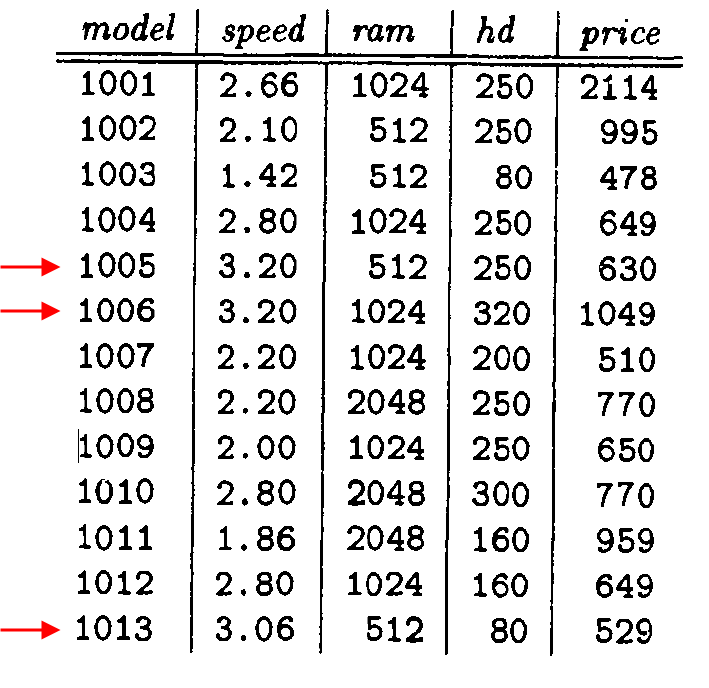
\includegraphics[width=0.4\linewidth]{images/worksheet_2_solution_2.png}
        \end{center}

        \bigskip

        \begin{mdframed}
            \underline{\textbf{Correct Solution:}}

            \bigskip

            \color{red}

            \textbf{Relational Algebra:}

            \bigskip

            $\pi_{model}(\sigma_{speed \geq 3.0}\text{(Movies)})$

            \bigskip

            \textbf{Query Result:}

            \bigskip

            \begin{tabular}{|c|}
                \hline
                model\\
                \hline
                1005\\
                \hline
                1006\\
                \hline
                1013\\
                \hline
            \end{tabular}
            \color{black}

            \bigskip

            Models 1005, 1006, 1013 have speed greater than 3.0
        \end{mdframed}

        \bigskip

        \underline{\textbf{Notes:}}

        \bigskip

        \begin{itemize}
            \item Select
            \begin{itemize}
                \item Is indicated by $\sigma$
                \item \textbf{Syntax:} $\sigma_{\text{QUERY}} \text{SCHEMA\_NAME}$
                \item e.g $\sigma_{length \geq 100 \textbf{ AND } studioName=`Fox'} \text{(Movies)}$

                \bigskip

                \begin{center}
                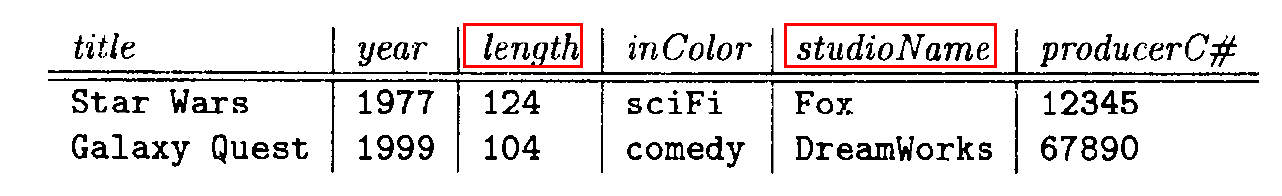
\includegraphics[width=\linewidth]{images/worksheet_2_solution_1.png}
                \end{center}
            \end{itemize}
        \end{itemize}

        \item

        $\pi_{maker}(\sigma_{hd \geq 100}(\text{Product} \bowtie \text{Laptop}))$

        \bigskip

        Makers $A,E,F,G$ make laptops with hard-disk of at least 100GB.

        \bigskip

        \begin{center}
        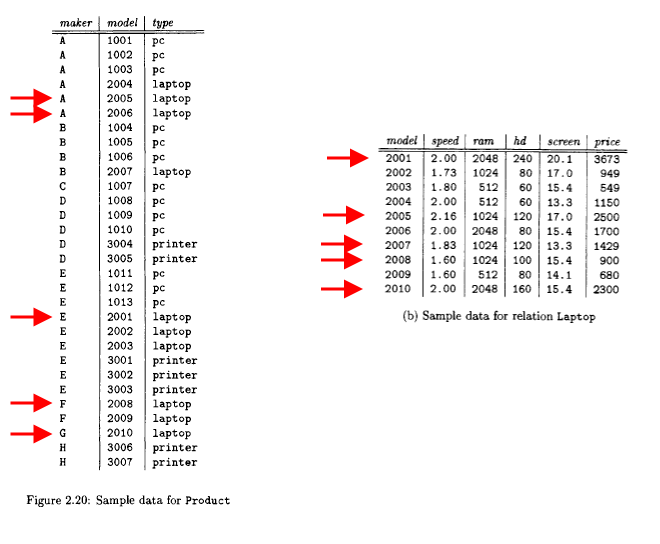
\includegraphics[width=\linewidth]{images/worksheet_2_solution_7.png}
        \end{center}

        \bigskip

        \begin{mdframed}
            \underline{\textbf{Correct Solution:}}

            \bigskip

            \color{red}

            \textbf{Relational Algebra:}

            \bigskip

            \color{black}

            $\pi_{maker}(\sigma_{hd \geq 100}(\text{Product} \bowtie \text{Laptop}))$

            \color{red}

            \bigskip

            \textbf{Query Result:}

            \bigskip

            \begin{tabular}{|c|}
                \hline
                maker\\
                \hline
                A\\
                \hline
                E\\
                \hline
                F\\
                \hline
                G\\
                \hline
            \end{tabular}
            \color{black}

            \bigskip

            Makers $A,E,F,G$ make laptops with hard-disk of at least 100GB.
        \end{mdframed}

        \bigskip

        \underline{\textbf{Notes:}}

        \bigskip

        \begin{itemize}
            \item Project
            \begin{itemize}
                \item \textbf{Syntax:} $\pi_{A_1, A_2, \cdots, A_n}$(Rel)
                \begin{itemize}
                    \item $A_1,\cdots,A_n$ represents attributes
                \end{itemize}
                \item Picks certain columns
                \item e.g

                \bigskip

                What are the titles and years of movies made by Fox that
                are at least 100 minutes long?

                \begin{align*}
                    \pi_{title,year}(\sigma_{length \geq 100 \textbf{ AND } studioName=`\textbf{Fox}'})(\text{Movies})
                \end{align*}
            \end{itemize}

            \item Cross-Product / Cartesian Product
            \begin{itemize}
                \item Combines two relations
                \item \textbf{Syntax:} Relation 1 $\times$ Relation 2
                \item e.g. Names and GPAs of students with $HS > 1000$ who applied
                to CS and were rejected

                \bigskip

                $ \pi_{sName, GPA}(\sigma_{Student.sID = Apply.sID \textbf{ AND }
                HS > 1000 \textbf{ AND } major = `cs' \textbf{ AND } dec = `R'})$(Student $\times$ Apply)

                \bigskip

                \begin{center}
                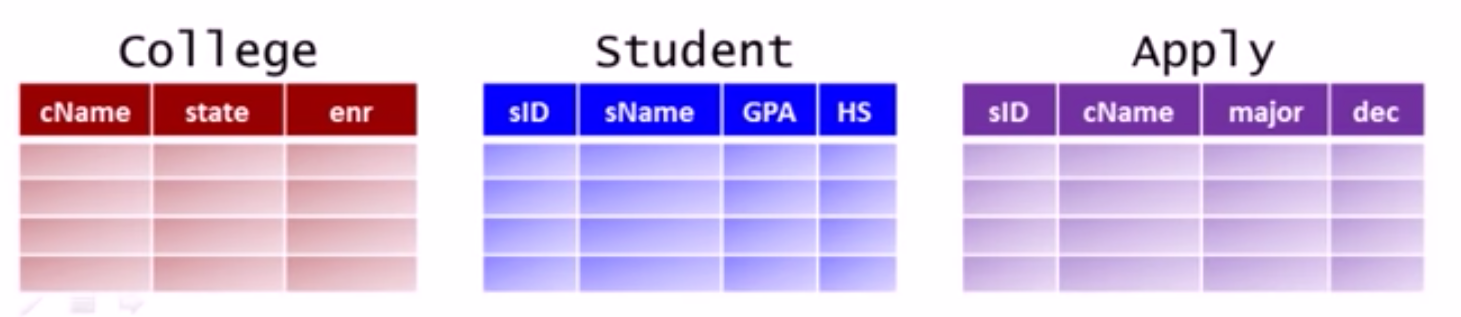
\includegraphics[width=\linewidth]{images/worksheet_2_solution_4.png}
                \end{center}
            \end{itemize}

            \item Natural Join
            \begin{itemize}
                \item Enforce equality on all attributes with the same name
                \item Eliminiate one copy of duplicate attributes
                \item Is symbolized by $\bowtie$
                \item \textbf{Syntax:} $\text{Relation 1} \bowtie \text{Relation 2}$
                \item e.g.

                \bigskip

                Names and GPAs of students with $HS > 1000$ who applied to CS and were
                rejected.

                \bigskip

                \begin{align*}
                    \pi_{sName,GPA} (\sigma_{HS > 1000 \textbf{ AND } major = `cs' \textbf{ AND } dec = `R'}\text{(Student $\bowtie$ Apply)})
                \end{align*}


                \begin{center}
                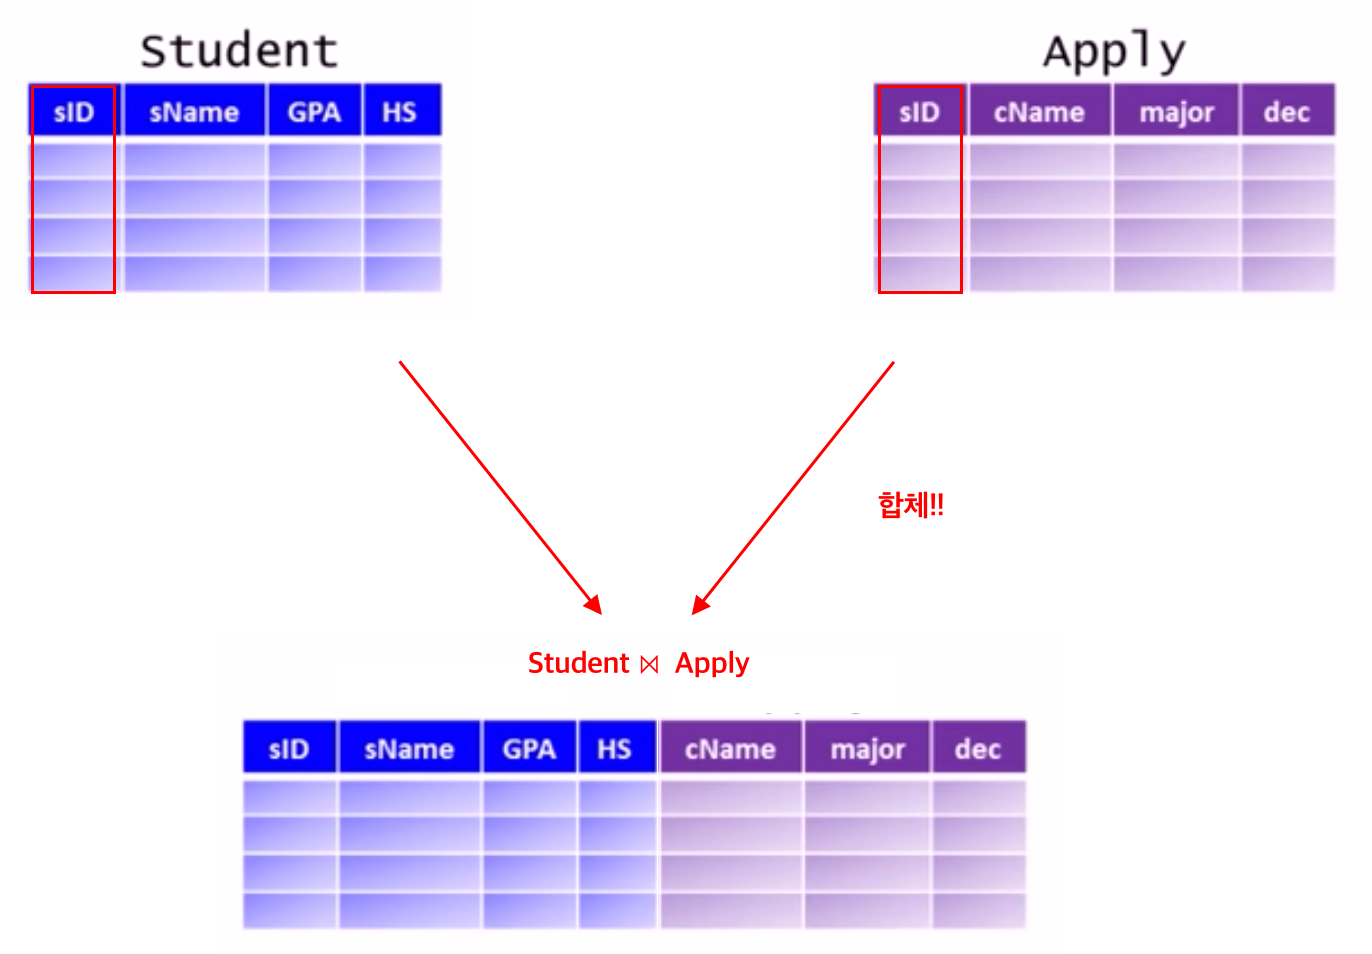
\includegraphics[width=\linewidth]{images/worksheet_2_solution_5.png}
                \end{center}

                \item e.g.2.

                \bigskip

                Names and GPAs of students with $HS > 1000$ who applied to CS
                at college with $enr > 20,000$ and were rejected

                \bigskip

                \begin{align*}
                    \begin{split}
                        &\pi_{sName,GPA} (\\
                        &\sigma_{HS > 1000 \textbf{ AND } enr > 20000 \textbf{ AND } major = `cs' \textbf{ AND } dec = `R'}\text{(Student $\bowtie$ (Apply $\bowtie$ College))}\\
                        &)
                    \end{split}
                \end{align*}

                \begin{center}
                
\includegraphics[width=\linewidth]{images/worksheet_2_solution_6.png}
                \end{center}

            \end{itemize}

            \item Union Operator
            \begin{itemize}
                \item \textbf{Syntax} $\text{R} \cup \text{S}$
                \item Is the set of elements that are in $R$ or $S$ or both.
                \item An element appears only once in the union even if it is
                    present in both $R$ and $S$.
                \item Is like \textbf{UNION} keyword in SQL
                \item e.g.

                \bigskip

                List of college and student names

                \begin{align*}
                    \pi_{cName}(\text{College}) \cup \pi_{sName} (\text{Student})
                \end{align*}
            \end{itemize}


            \item Difference Operator
            \begin{itemize}
                \item \textbf{Syntax:} $R - S$
                \item Is also called the \textit{difference} of $R$ and $S$
                \item is the set of elements that are in $R$ but not in $S$.
                \item Is like \textbf{EXCEPT} keyword in SQL
                \item e.g.

                \bigskip

                IDs and names of students who didn't apply anywhere

                \begin{align*}
                    \pi_{sID} (\text{Student}) - \pi_{sID}(\text{Apply})
                \end{align*}
            \end{itemize}

            \item Intersection Operator
            \begin{itemize}
                \item \textbf{Syntax:} $R \cap S$
                \item Is also canned the \textit{intersection} of $R$ and $S$
                \item Is the set of elements that are in both $R$ and $S$
                \item e.g.

                \bigskip

                Names that are both a college name and a student name

                \bigskip

                \begin{align*}
                    \pi_{cName} (\text{College}) - \pi_{sName}(\text{Student})
                \end{align*}
            \end{itemize}
        \end{itemize}

        \item

        \begin{align}
            \begin{split}
            &\pi_{model,price}(\sigma_{maker=`\text{B}'}(\\
            &\text{Product} \bowtie (\pi_{model,price}(\text{Laptop}) \cup \pi_{model,price}(\text{PC}) \cup \pi_{model,price}(\text{Printer})\\
            &))
            \end{split}
        \end{align}

        \bigskip

        The price and model number of all products made by manufacturer B are


        \begin{enumerate}[1.]
            \item model 1004, price 649
            \item model 1005, price 630
            \item model 1006, price 1049
            \item model 2007, price 1429
        \end{enumerate}

        \begin{center}
        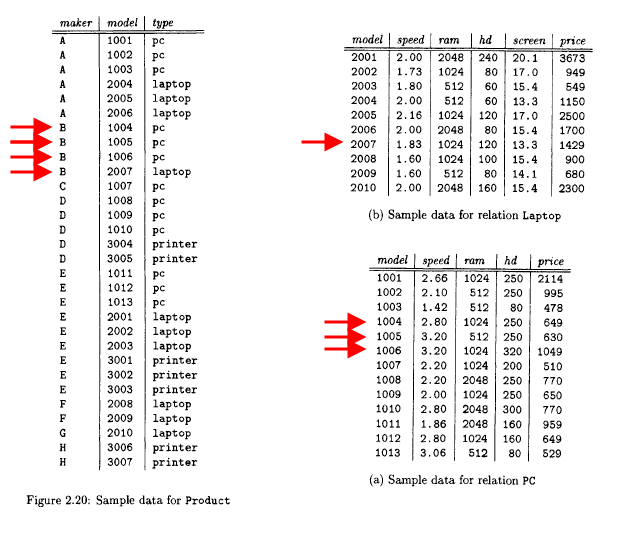
\includegraphics[width=\linewidth]{images/worksheet_2_solution_8.png}
        \end{center}

        \bigskip

        \begin{mdframed}
            \underline{\textbf{Correct Solution:}}

            \bigskip

            \color{red}

            \textbf{Relational Algebra:}

            \bigskip

            \color{black}

            \begin{align}
                \begin{split}
                &\pi_{model,price}(\sigma_{maker=`\text{B}'}(\\
                &\text{Product} \bowtie (\pi_{model,price}(\text{Laptop}) \cup \pi_{model,price}(\text{PC}) \cup \pi_{model,price}(\text{Printer})\\
                &))
                \end{split}
            \end{align}

            \color{red}

            \bigskip

            \textbf{Query Result:}

            \bigskip

            \begin{tabular}{|c|c|}
                \hline
                model   &   price\\
                \hline
                1004    &   649\\
                \hline
                1005    &   630\\
                \hline
                1006    &   1049\\
                \hline
                2007    &   1429\\
                \hline
            \end{tabular}
            \color{black}

            \bigskip

            The price and model number of all products made by manufacturer B are

            \begin{enumerate}[1.]
                \item model 1004, price 649
                \item model 1005, price 630
                \item model 1006, price 1049
                \item model 2007, price 1429
            \end{enumerate}
        \end{mdframed}



        \item $\pi_{model} (\sigma_{color = \text{true} \textbf{ AND } type=`\text{laser}'}(\text{Printer}))$

        \bigskip

        Model 3003, and 3007 are color laster printers

        \begin{center}
        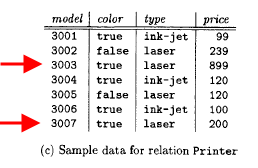
\includegraphics[width=0.4\linewidth]{images/worksheet_2_solution_9.png}
        \end{center}

        \bigskip

        \begin{mdframed}
            \underline{\textbf{Correct Solution:}}

            \bigskip

            \color{red}

            \textbf{Relational Algebra:}

            \bigskip

            \color{black}

            $\pi_{model} (\sigma_{color = \text{true} \textbf{ AND } type=`\text{laser}'}(\text{Printer}))$

            \color{red}

            \bigskip

            \textbf{Query Result:}

            \bigskip

            \begin{tabular}{|c|}
                \hline
                model\\
                \hline
                3003\\
                \hline
                3007\\
                \hline
            \end{tabular}
            \color{black}

            \bigskip

            Model 3003, and 3007 are color laster printers
        \end{mdframed}

        \item $\pi_{maker}(\text{Product} \bowtie (\pi_{model} (\text{Laptops}) - \pi_{model} (\text{PC})))$

        \bigskip

        Manufacturers $F$ and $G$ produce laptops but not PCs

        \begin{center}
        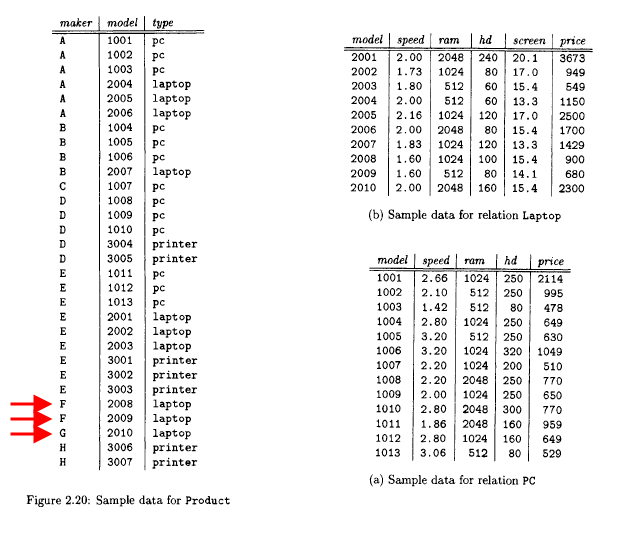
\includegraphics[width=\linewidth]{images/worksheet_2_solution_10.png}
        \end{center}

        \bigskip

        \begin{mdframed}
            \underline{\textbf{Correct Solution:}}

            \bigskip

            \color{red}

            \textbf{Relational Algebra:}

            \bigskip

            $\color{red}\pi_{maker}(\sigma_{type = `\text{laptop}' \textbf{ AND } type <> `\text{PC}'}(\text{Product}))$

            \bigskip

            \textbf{Query Result:}

            \bigskip

            \begin{tabular}{|c|}
                \hline
                maker\\
                \hline
                F\\
                \hline
                G\\
                \hline
            \end{tabular}
            \color{black}

            \bigskip

            Manufacturers $F$ and $G$ produce laptops but not PCs
        \end{mdframed}

        \bigskip

        \underline{\textbf{Notes:}}

        \bigskip

        \begin{itemize}
            \item `$<>$' Means `NOT EQUAL' in relational algebra
            \item Relational algebra inclues \underline{six} comparison operators
            ($=,<>,<,>,\geq,\leq)$ $^{[1]}$
            \item Relational projection (i.e. $\pi$) \underline{always} return
            distinct tuples $^{[2]}$
        \end{itemize}

        \bigskip

        \underline{\textbf{Reference:}}

        \bigskip

        \begin{enumerate}[1)]
            \item Radboud University: IS0 - Relational Languages, \href{http://www.cs.ru.nl/~gerp/IS0/sheets/IS0_Relationele_Algebra_SQL2.pdf}{link}
            \item Stack Overflow: Selecting DISTINCT rows in relational algebra, \href{https://stackoverflow.com/questions/4775728/selecting-distinct-rows-in-relational-algebra}{link}
        \end{enumerate}



        \item $\pi_{hd}(\sigma_{hd = hd2}(\pi_{hd}(PC) \times \rho_{\pi_{hd}(PC)(hd2)}(\pi_{hd}(PC))))$

        \bigskip

        \textbf{Query Result:}

        \bigskip

        \begin{tabular}{|c|}
            \hline
            hd\\
            \hline
            250\\
            \hline
            80\\
            \hline
            160\\
            \hline
        \end{tabular}

        \bigskip

        \begin{mdframed}
            \underline{\textbf{Correct Solution:}}

            \bigskip

            \color{red}

            \textbf{Relational Algebra:}

            \bigskip

            $\pi_{hd}(\sigma_{hd = hd2}(\pi_{hd}(PC) \times \pi_{hd2}(\rho_{hd \to hd2}(PC))))$

            \bigskip

            \textbf{Query Result:}

            \bigskip

            \begin{tabular}{|c|}
                \hline
                hd\\
                \hline
                250\\
                \hline
                80\\
                \hline
                160\\
                \hline
            \end{tabular}
            \color{black}
        \end{mdframed}

    \end{enumerate}

    \item

    \begin{enumerate}[a)]
        \item

        \textbf{Answer:}

        \bigskip

        \begin{center}
        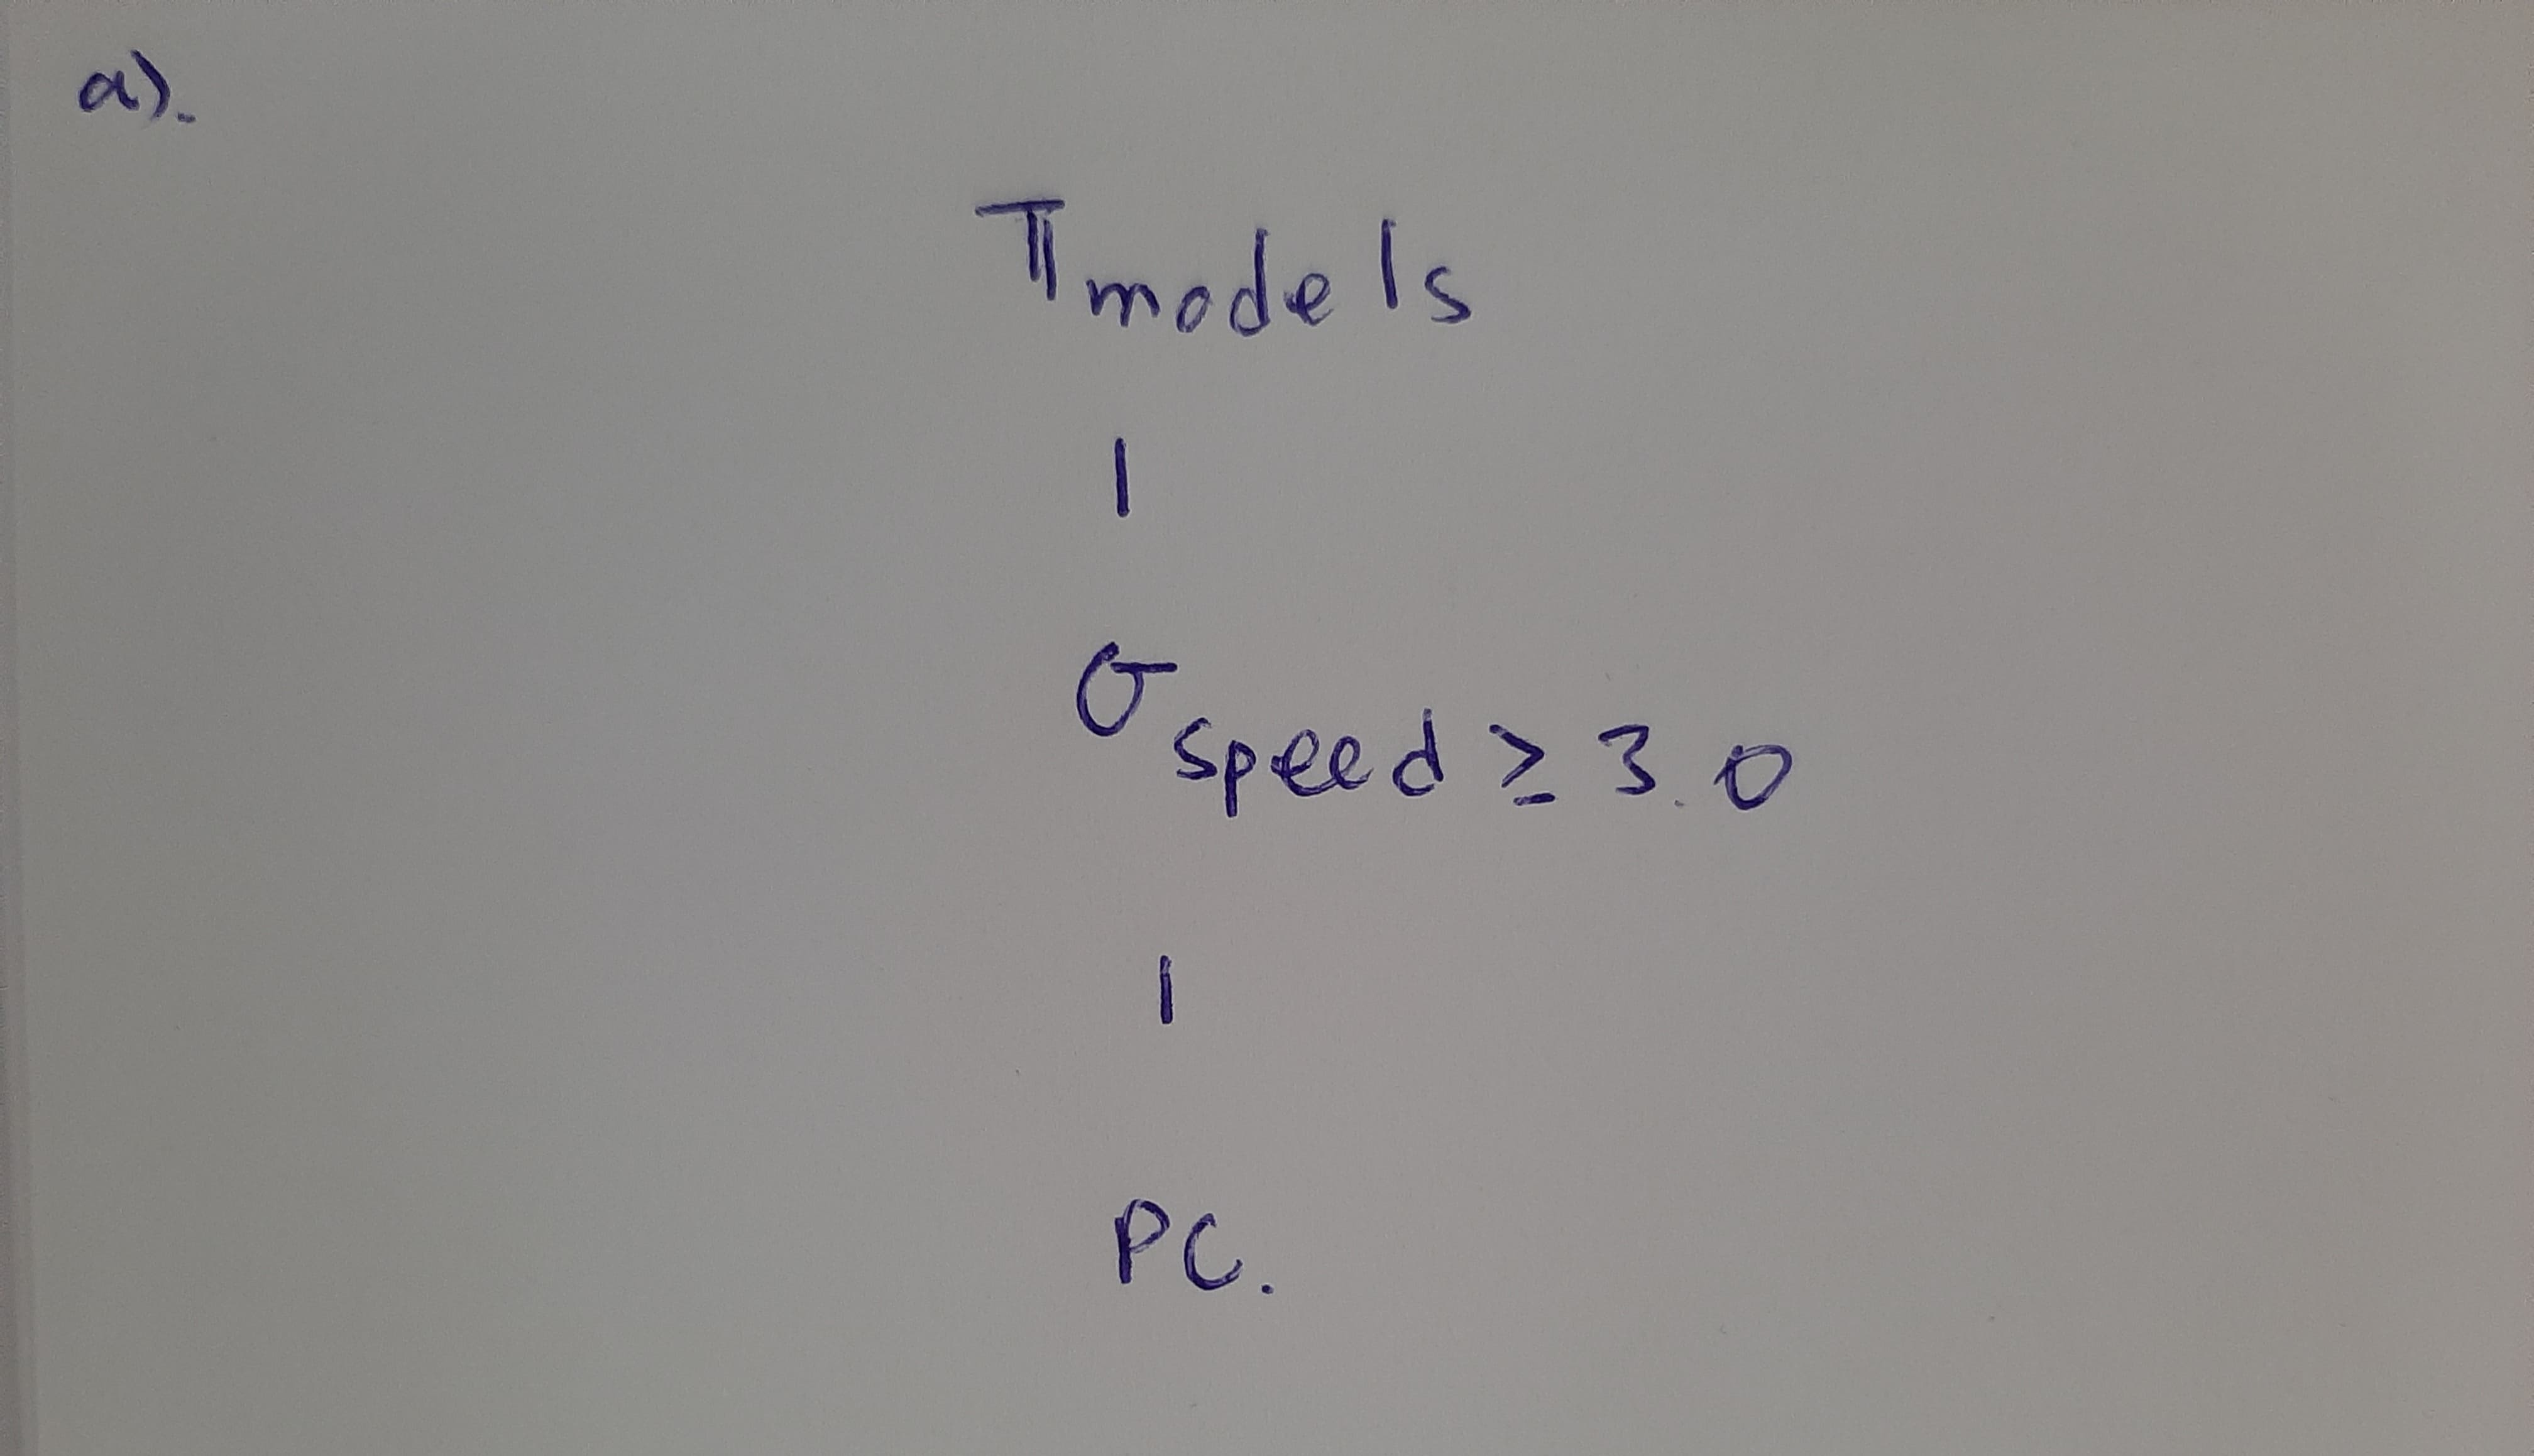
\includegraphics[width=0.7\linewidth]{images/worksheet_2_solution_11.jpg}
        \end{center}

        \item

        \textbf{Answer:}

        \bigskip

        \begin{center}
        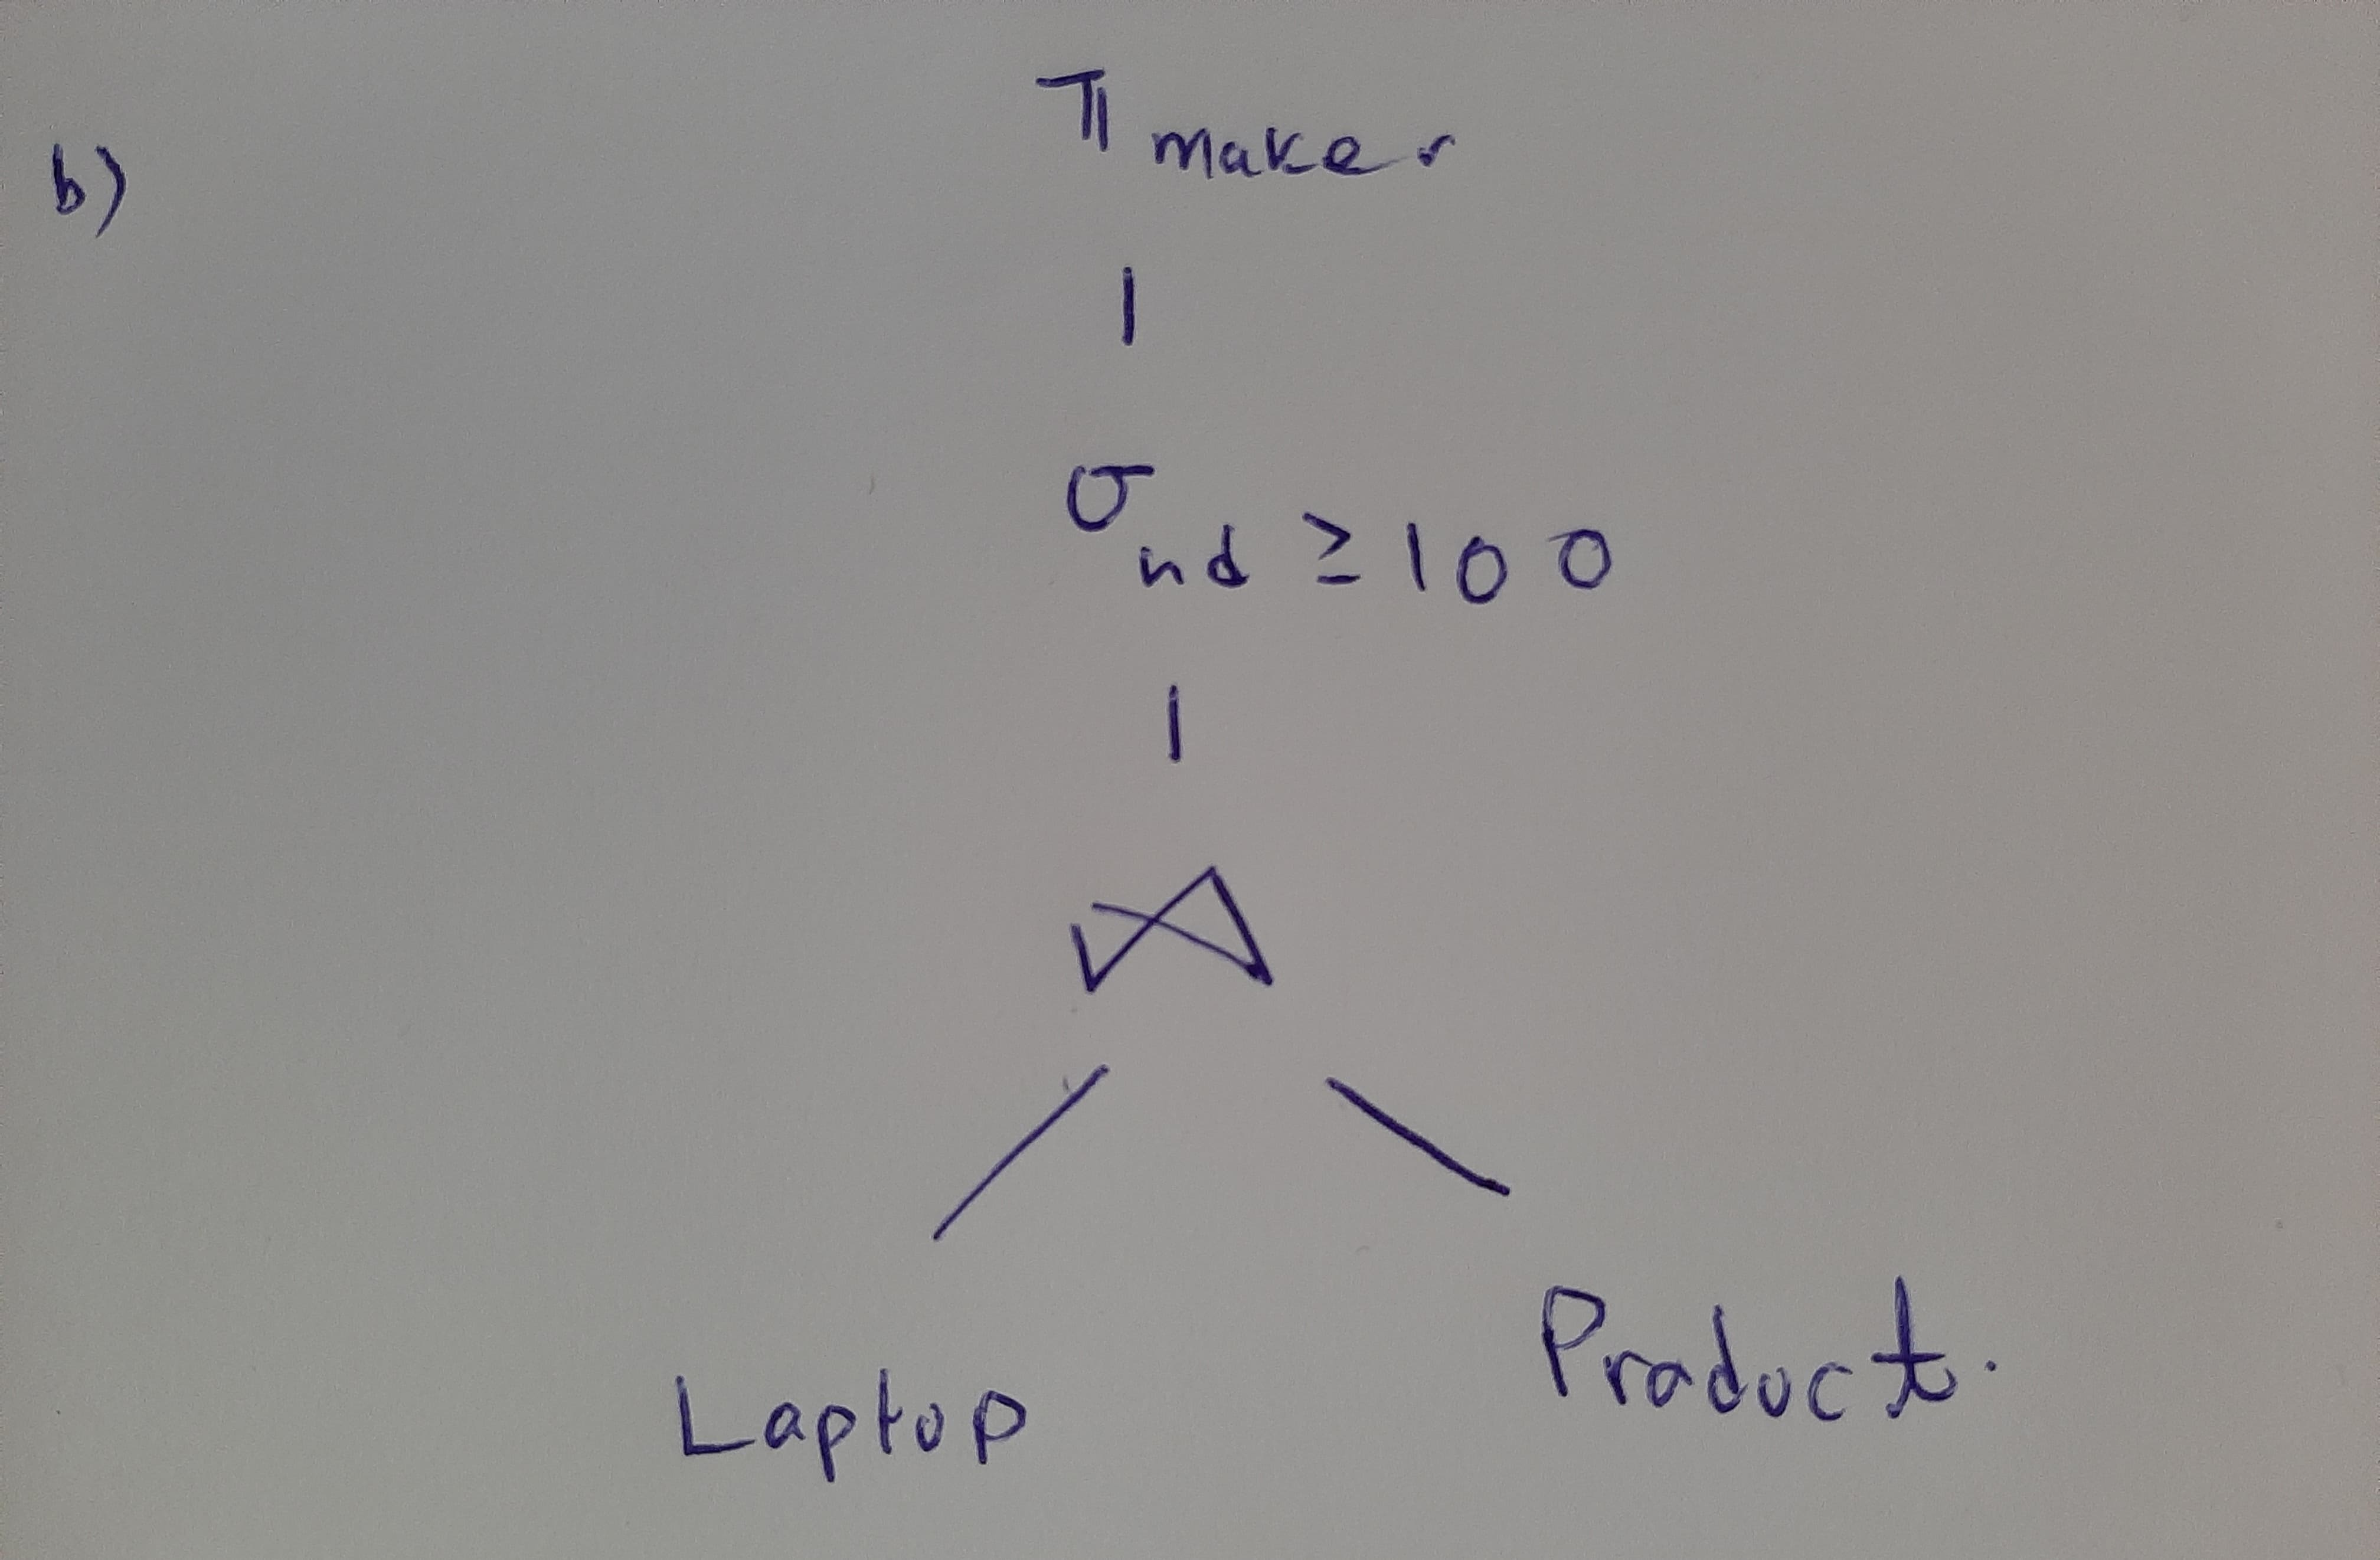
\includegraphics[width=0.7\linewidth]{images/worksheet_2_solution_12.jpg}
        \end{center}

        \item

        \textbf{Answer:}

        \bigskip

        \begin{center}
        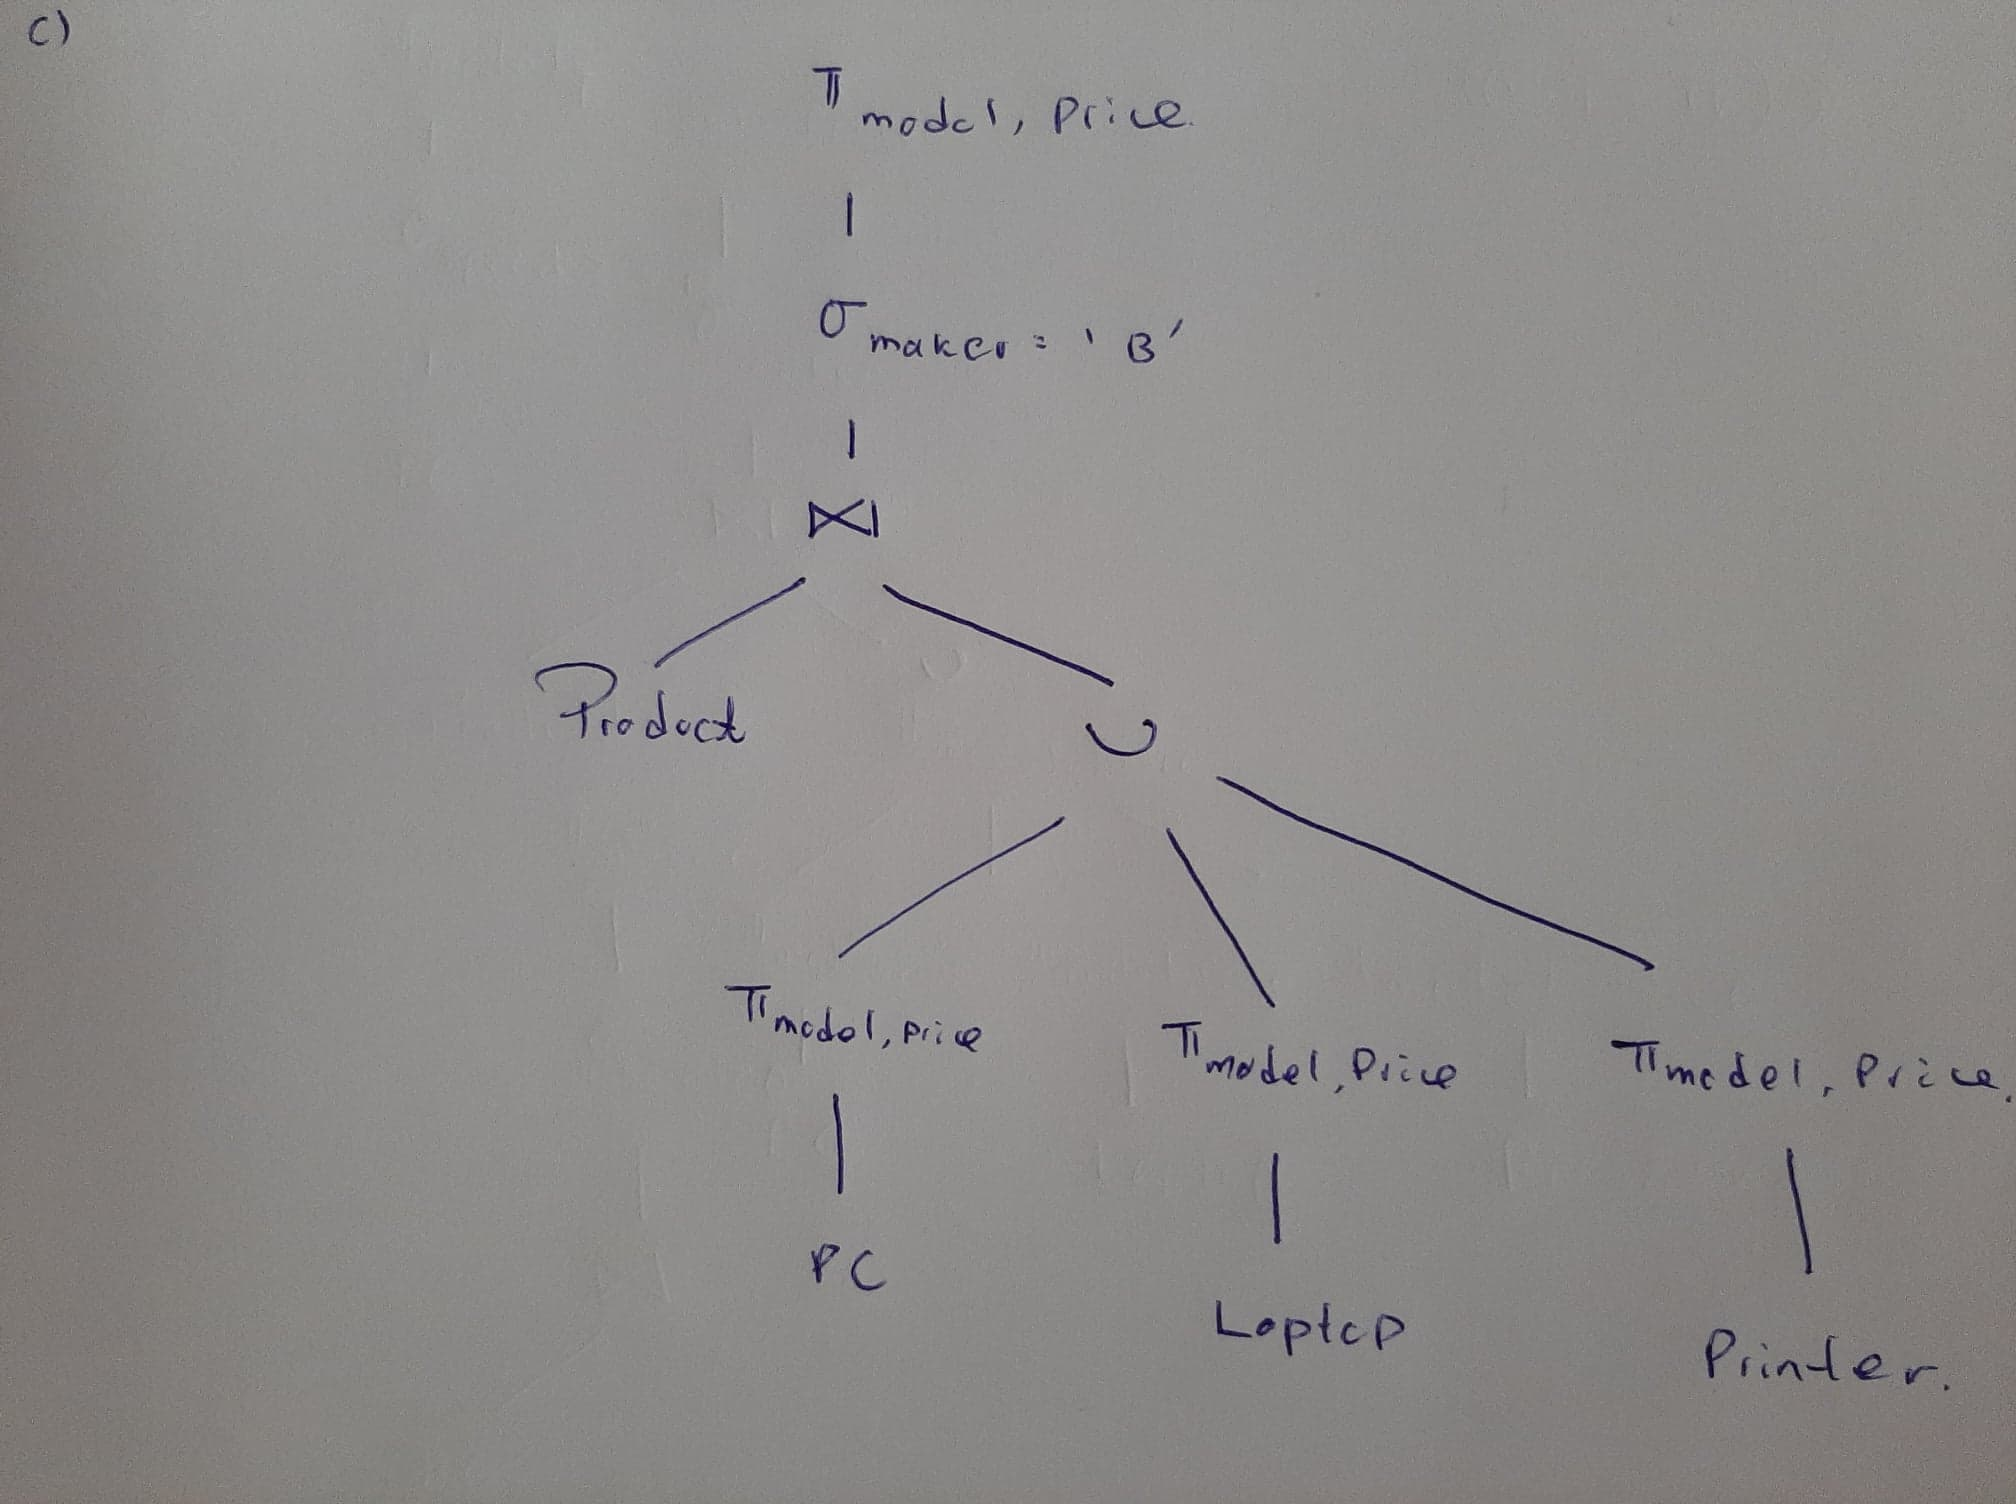
\includegraphics[width=0.7\linewidth]{images/worksheet_2_solution_13.jpg}
        \end{center}

        \item

        \textbf{Answer:}

        \bigskip

        \begin{center}
        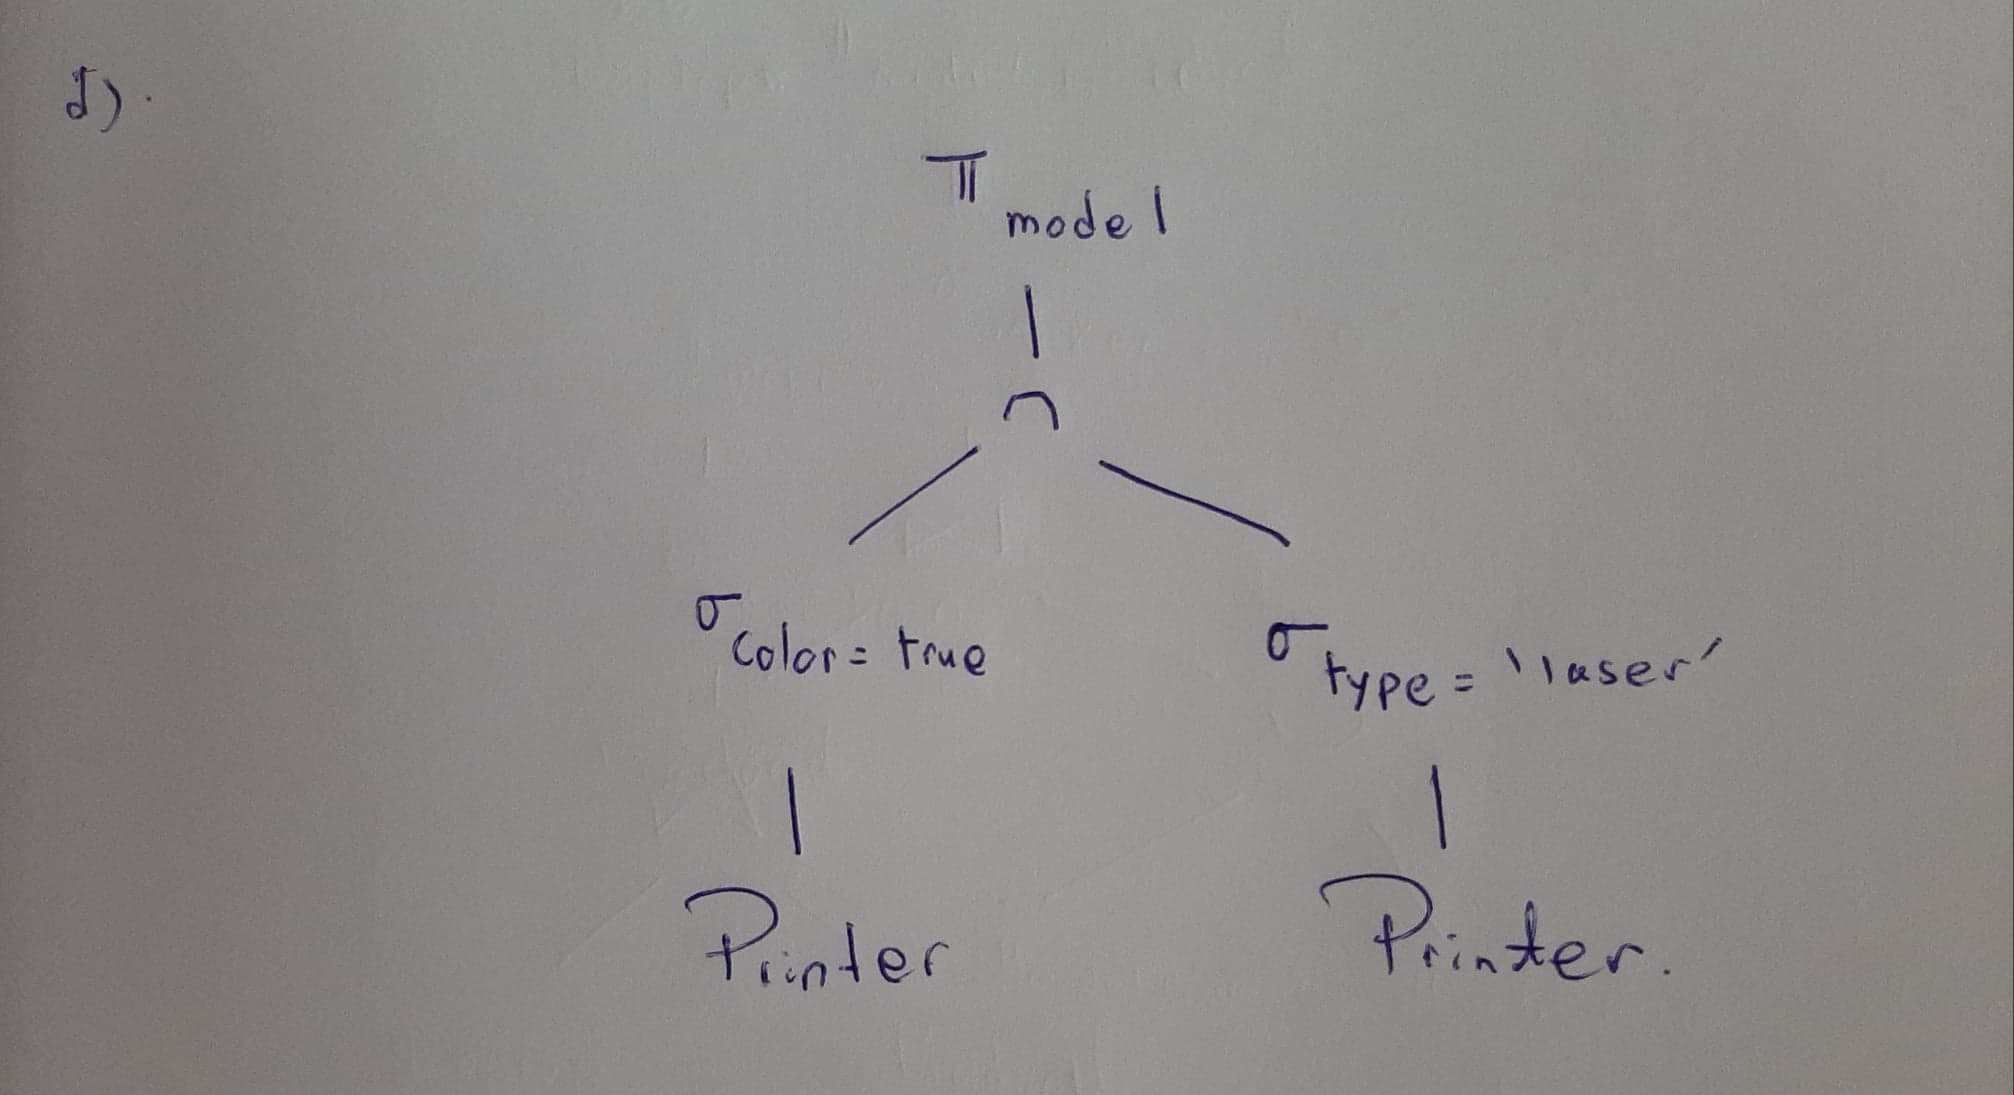
\includegraphics[width=0.7\linewidth]{images/worksheet_2_solution_14.jpg}
        \end{center}

        \item

        \textbf{Answer:}

        \bigskip

        \begin{center}
        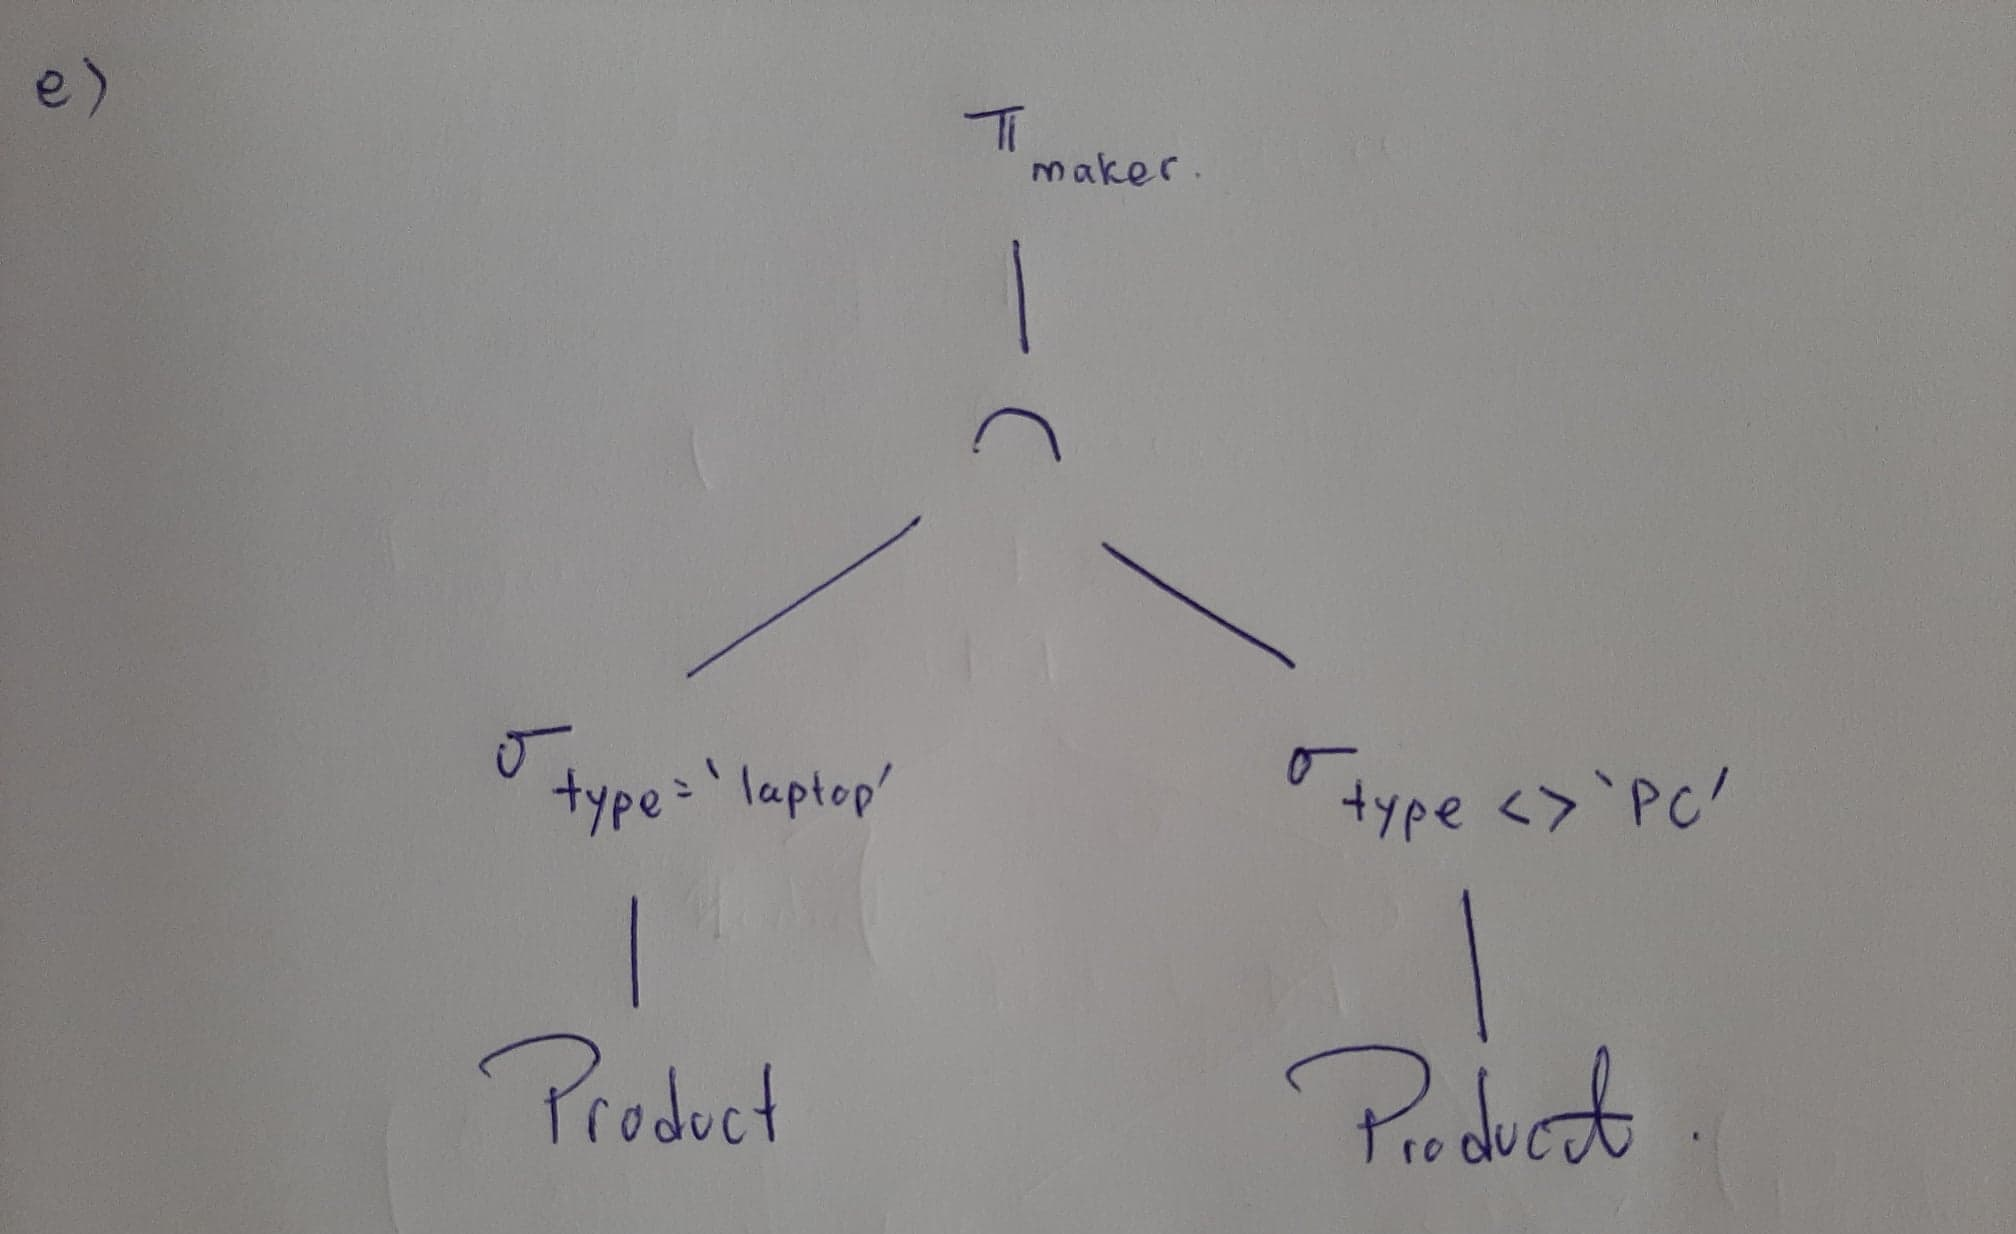
\includegraphics[width=0.7\linewidth]{images/worksheet_2_solution_15.jpg}
        \end{center}

        \item

        \textbf{Answer:}

        \bigskip

        \begin{center}
        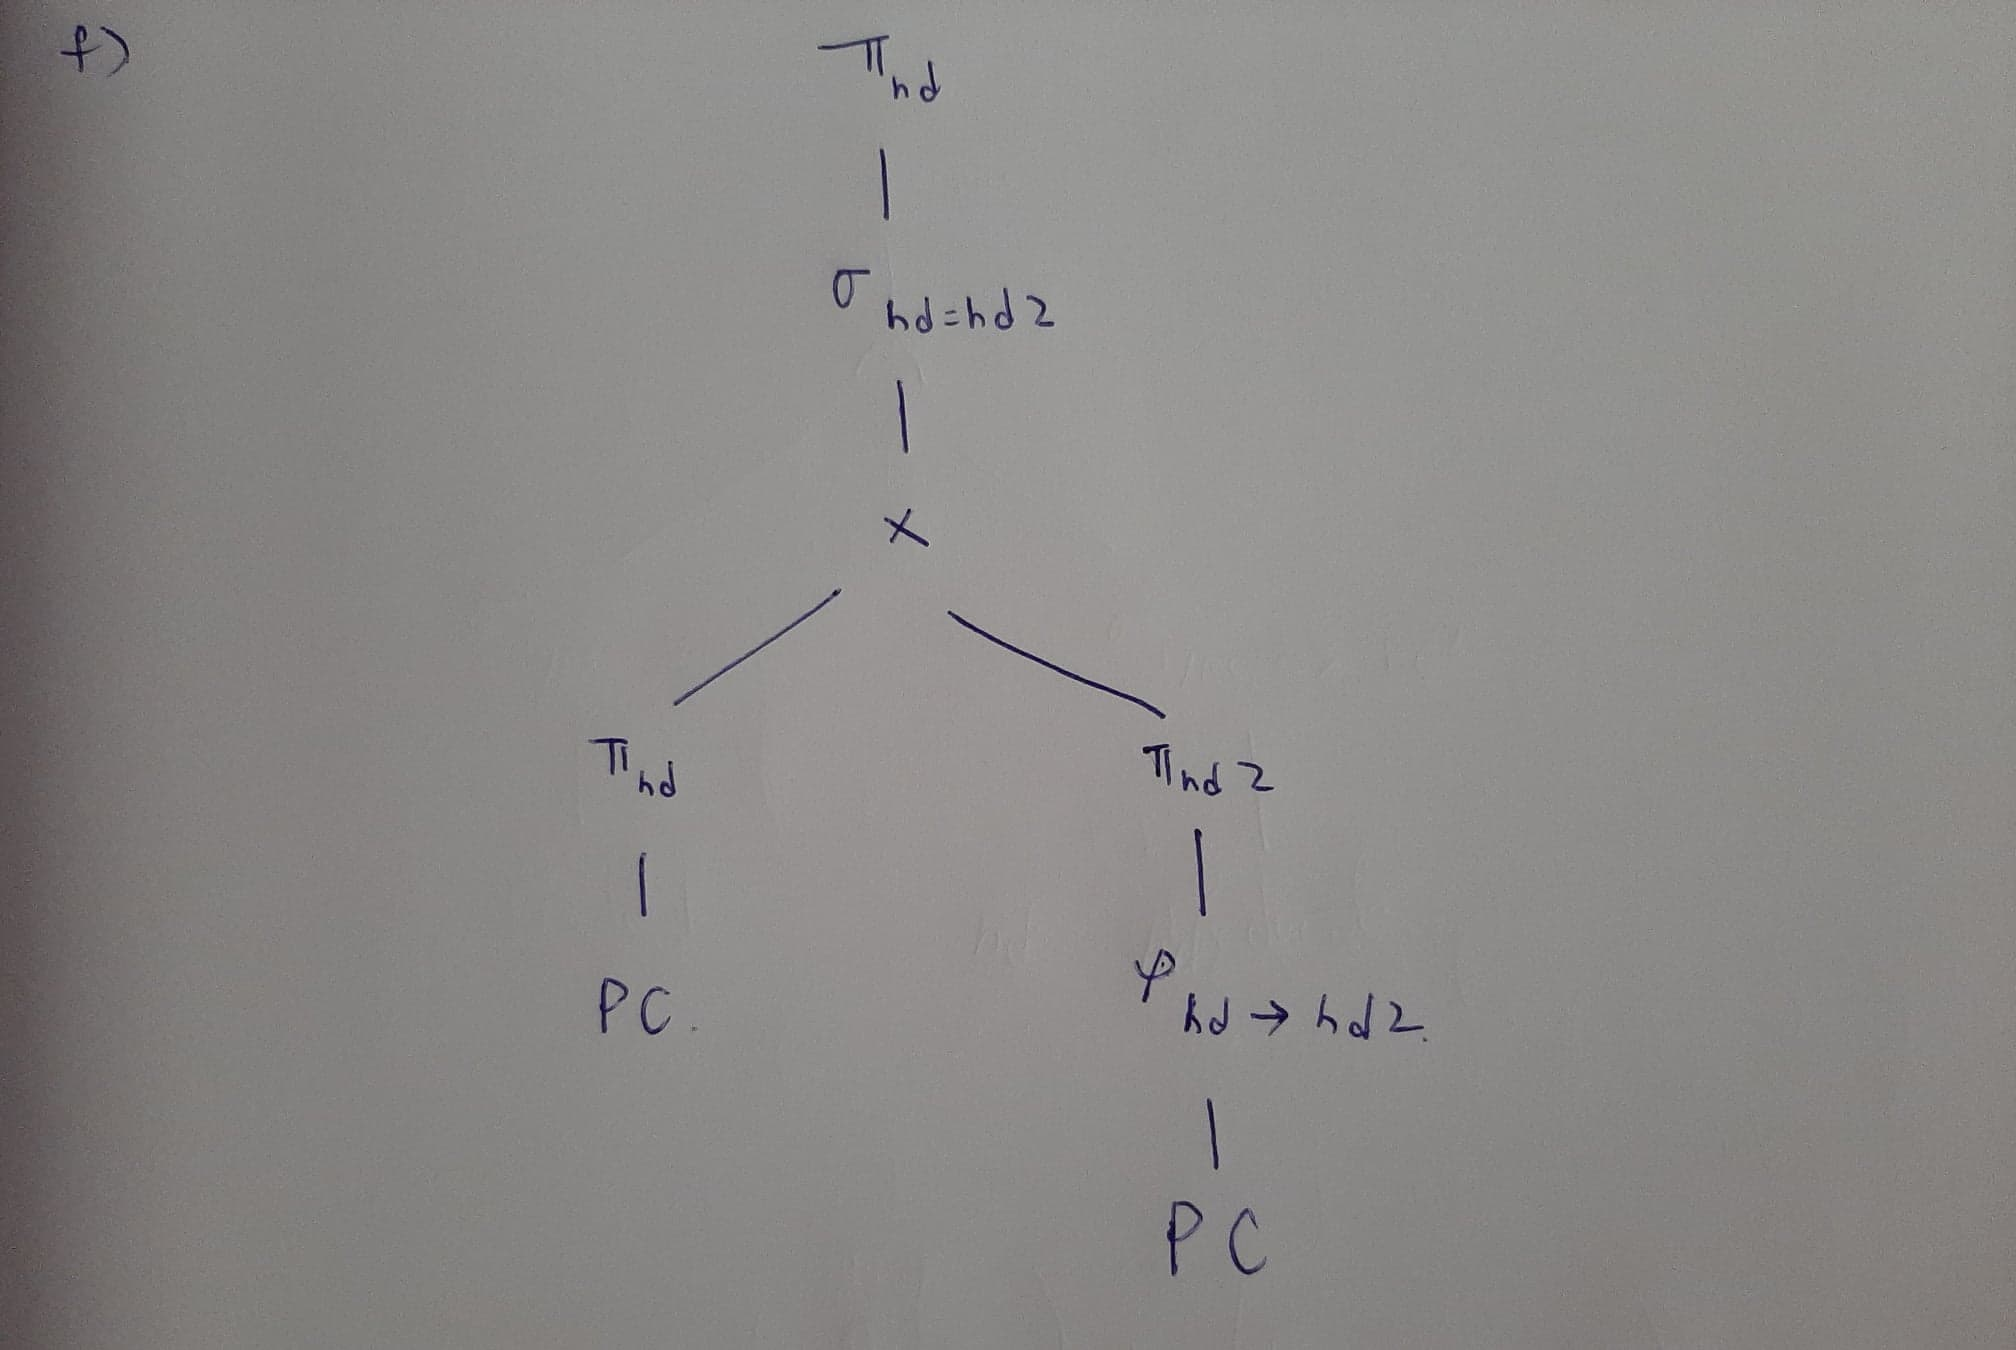
\includegraphics[width=0.7\linewidth]{images/worksheet_2_solution_16.jpg}
        \end{center}

    \end{enumerate}

    \item

    \begin{enumerate}[a)]
        \item

        \textbf{Relational Algebra:}

        \bigskip

        $\pi_{class,countries}(\sigma_{bore \geq 16}(\text{Classes}))$

        \bigskip

        \textbf{Query Result:}

        \bigskip

        \begin{tabular}{|c|c|}
            \hline
            class   &   countries\\
            \hline
            Iowa    &   USA   \\
            \hline
            North Carolina  &   USA\\
            \hline
            Yamato  &   Japan\\
            \hline
        \end{tabular}

        \item

        \textbf{Relational Algebra:}

        \bigskip

        $\sigma_{launched < 1921}(\text{Ships})$

        \bigskip

        \textbf{Query Result:}

        \bigskip

        \begin{tabular}{|c|c|c|}
            \hline
            name    &   class   & launched\\
            \hline
            Haruna  &   Kongo   & 1915\\
            \hline
            Hiei    &   Kongo   & 1914\\
            \hline
            Kirishima   & Kongo & 1915\\
            \hline
            Kongo       & Kongo & 1913\\
            \hline
            Ramillies   & Revenge & 1917\\
            \hline
            Renown      & Renown & 1916\\
            \hline
            Repulse     & Renown & 1916\\
            \hline
            Resolution  & Revenge & 1916\\
            \hline
            Revenge     & Revenge & 1916\\
            \hline
            Royal Oak   & Revenge & 1916\\
            \hline
            Royal Sovereign & Revenge & 1916\\
            \hline
            Tennessee   & Tennessee & 1920\\
            \hline
        \end{tabular}

        \item

        \textbf{Relational Algebra:}

        \bigskip

        $\sigma_{battle=`\text{Denmark Strait}' \textbf{ AND } result=`\text{sunk}'}(\text{Outcome})$

        \bigskip

        \textbf{Query Result:}

        \bigskip

        \begin{tabular}{|c|c|c|}
            \hline
            Ships   &   battle  & result\\
            \hline
            Bismark &   Denmark Strait  & sunk\\
            \hline
            Hood    &   Denmark Strait  & sunk\\
            \hline
        \end{tabular}

        \item

        \textbf{Relational Algebra:}

        \bigskip

        $Classes \bowtie_{displacement > 35,000} Ships$

        \bigskip

        \textbf{Query Result:}

        \bigskip

        \resizebox{\textwidth}{!}{%
        \begin{tabular}{|c|c|c|c|c|c|c|c|}
            \hline
            name    &   class   &   launched    &   type    &   country &   numGuns   &   bore  &   displacement\\
            \hline
            Iowa    &   Iowa    &   1943    &   bb  &   USA &   9   &   16  &   46000\\
            \hline
            Missouri    &   Iowa    &   1944    &   bb  &   USA &   9   &   16  &   46000\\
            \hline
            New Jersey  &   Iowa    &   1943    &   bb  &   USA &   9   &   16  &   46000\\
            \hline
            Wisconsin   &   Iowa    &   1944    &   bb  &   USA &   9   &   16  &   46000\\
            \hline
            Haruna  &   Kongo   &   1915    &   bc  &   Japan   &   8   &   14  &   32000\\
            \hline
            Hiei  &   Kongo   &   1914    &   bc  &   Japan   &   8   &   14  &   32000\\
            \hline
            Kirishima  &   Kongo   &   1915    &   bc  &   Japan   &   8   &   14  &   32000\\
            \hline
            Kongo  &   Kongo   &   1913    &   bc  &   Japan   &   8   &   14  &   32000\\
            \hline
            Kongo  &   Kongo   &   1913    &   bc  &   Japan   &   8   &   14  &   32000\\
            \hline
            North Carolina  &   North Carolina    &   1941    &   bb  &   USA &   9   &   16  &   37000\\
            \hline
            Washington  &   North Carolina    &   1941    &   bb  &   USA &   9   &   16  &   37000\\
            \hline
            Washington  &   North Carolina    &   1941    &   bb  &   USA &   9   &   16  &   37000\\
            \hline
            Renown  &   Renown    &   1916    &   bc  &   Gt. Britain   &   6   &   15  &   42000\\
            \hline
            Repulse  &   Repulse    &   1916    &   bc  &   Gt. Britain   &   6   &   15  &   42000\\
            \hline
            Ramillies  &   Revenge    &   1917    &   bb  &   Gt. Britain   &   8   &   15  &   29000\\
            \hline
            Resolution  &   Revenge    &   1916    &   bb  &   Gt. Britain   &   8   &   15  &   29000\\
            \hline
            Revenge  &   Revenge    &   1916    &   bb  &   Gt. Britain   &   8   &   15  &   29000\\
            \hline
            Royal Oak  &   Revenge    &   1916    &   bb  &   Gt. Britain   &   8   &   15  &   29000\\
            \hline
            Royal Sovereign  &   Revenge    &   1916    &   bb  &   Gt. Britain   &   8   &   15  &   29000\\
            \hline
            California  &   Tennessee    &   1921    &   bb  &   USA   &   12   &   14  &   32000\\
            \hline
            Yamato  &   Yamato    &   1941    &   bb  &   Japan   &   9   &   18  &   65000\\
            \hline
        \end{tabular}}


        \bigskip

        \begin{mdframed}
            \underline{\textbf{Correct Solution:}}

            \bigskip

            \textbf{Relational Algebra:}

            \bigskip

            $Classes \bowtie_{displacement > 35,000} Ships$

            \bigskip

            \textbf{Query Result:}

            \bigskip

            \resizebox{\textwidth}{!}{%
            \begin{tabular}{|c|c|c|c|c|c|c|c|}
                \hline
                name    &   class   &   launched    &   type    &   country &   numGuns   &   bore  &   displacement\\
                \hline
                Iowa    &   Iowa    &   1943    &   bb  &   USA &   9   &   16  &   46000\\
                \hline
                Missouri    &   Iowa    &   1944    &   bb  &   USA &   9   &   16  &   46000\\
                \hline
                New Jersey  &   Iowa    &   1943    &   bb  &   USA &   9   &   16  &   46000\\
                \hline
                Wisconsin   &   Iowa    &   1944    &   bb  &   USA &   9   &   16  &   46000\\
                \hline
                Haruna  &   Kongo   &   1915    &   bc  &   Japan   &   8   &   14  &   32000\\
                \hline
                Hiei  &   Kongo   &   1914    &   bc  &   Japan   &   8   &   14  &   32000\\
                \hline
                Kirishima  &   Kongo   &   1915    &   bc  &   Japan   &   8   &   14  &   32000\\
                \hline
                North Carolina  &   North Carolina    &   1941    &   bb  &   USA &   9   &   16  &   37000\\
                \hline
                Washington  &   North Carolina    &   1941    &   bb  &   USA &   9   &   16  &   37000\\
                \hline
                Washington  &   North Carolina    &   1941    &   bb  &   USA &   9   &   16  &   37000\\
                \hline
                Yamato  &   Yamato    &   1941    &   bb  &   Japan   &   9   &   18  &   65000\\
                \hline
                Musashi  &   Yamato    &   1942    &   bb  &   Japan   &   9   &   18  &   65000\\
                \hline
            \end{tabular}}

        \end{mdframed}

        \item

        \textbf{Relational Algebra:}

        \bigskip

        $\pi_{name,displacement,numGuns}(\text{Classes} \bowtie_{battle=`\text{Guadalcanal}} (\rho_{ship \to name} (\text{Outcomes} \bowtie \text{Ships})))$

        \bigskip

        \textbf{Query Result:}

        \bigskip

        \begin{tabular}{|c|c|c|}
            \hline
            name    &   displacement    &   numGuns\\
            \hline
            Kirishima   &   32000   &   8\\
            \hline
            Washington   &   37000   &   9\\
            \hline
        \end{tabular}

        \bigskip

        \item

        \textbf{Relational Algebra:}

        \bigskip

        $\pi_{name}(\rho_{ship \to name}(\text{Outcomes})) \cup \pi_{name}(\text{Ships})$

        \bigskip

        \textbf{Query Result:}

        \bigskip

        \begin{tabular}{|c|}
            \hline
            name\\
            \hline
            Arizona\\
            \hline
            Bismark\\
            \hline
            California\\
            \hline
            Duke of York\\
            \hline
            Fuso\\
            \hline
            Hood\\
            \hline
            King George V\\
            \hline
            Kirishima\\
            \hline
            Prince of Wales\\
            \hline
            Rodney\\
            \hline
            Scharnhorst\\
            \hline
            South Dakota\\
            \hline
            Tennessee\\
            \hline
            Washington\\
            \hline
            West Virginia\\
            \hline
            Yamashiro\\
            \hline
            Haruna\\
            \hline
            Hiei\\
            \hline
            Iowa\\
            \hline
            Kongo\\
            \hline
            Missouri\\
            \hline
            Musashi\\
            \hline
            New Jersey\\
            \hline
            North Carolina\\
            \hline
            Ramillies\\
            \hline
            Renown\\
            \hline
            Repulse\\
            \hline
            Resolution\\
            \hline
            Revenge\\
            \hline
            Royal Oak\\
            \hline
            Royal Sovereign\\
            \hline
            Wisconsin\\
            \hline
            Yamato\\
            \hline
        \end{tabular}

        \item Omitted for now

        \item

        \textbf{Relational Algebra:}

        \bigskip

        $\pi_{country}(\sigma_{type = `\text{bb}'} (\text{Classes})) \cap \pi_{country}(\sigma_{type = `\text{bc}'}(\text{Classes}))$

        \bigskip

        \textbf{Query Result:}

        \bigskip

        \begin{tabular}{|c|}
            \hline
            country\\
            \hline
            Japan\\
            \hline
            Gt. Britain\\
            \hline
        \end{tabular}

        \item Omitted for now

    \end{enumerate}

    \item

    \begin{enumerate}[a)]
        \item

        \textbf{Answer:}

        \bigskip

        \begin{center}
        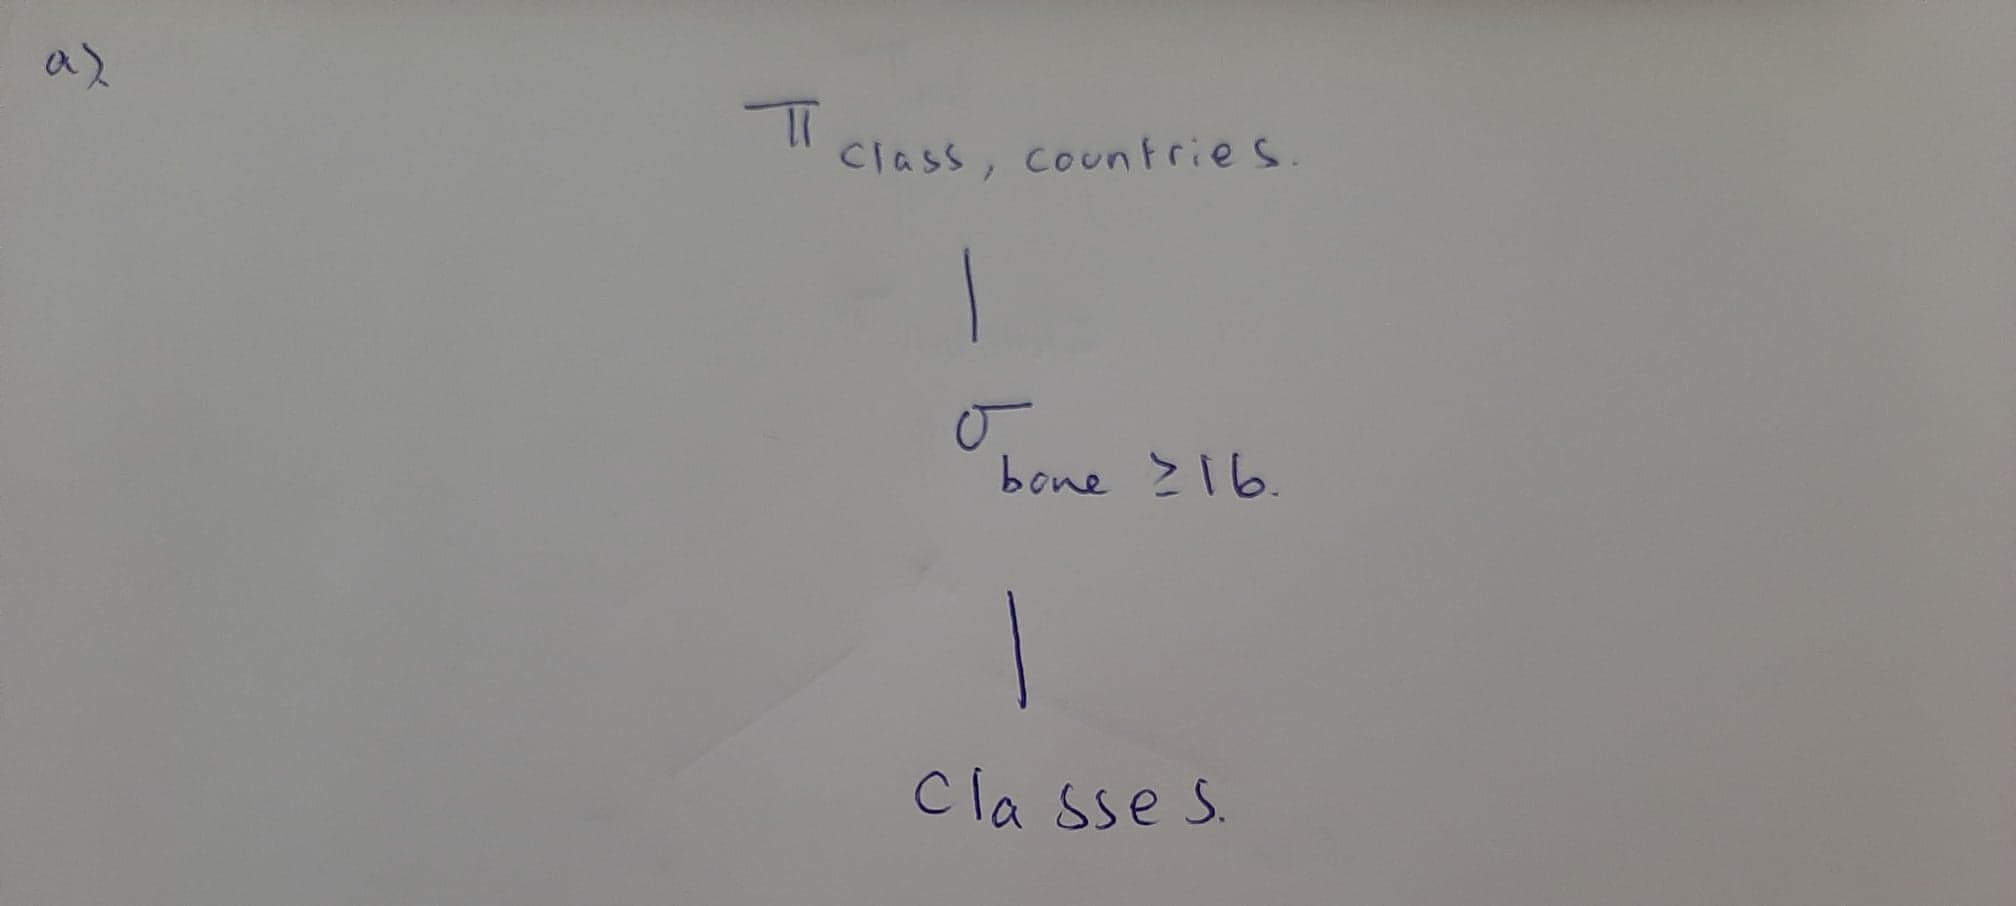
\includegraphics[width=0.7\linewidth]{images/worksheet_2_solution_17.jpg}
        \end{center}

        \item

        \textbf{Answer:}

        \bigskip

        \begin{center}
        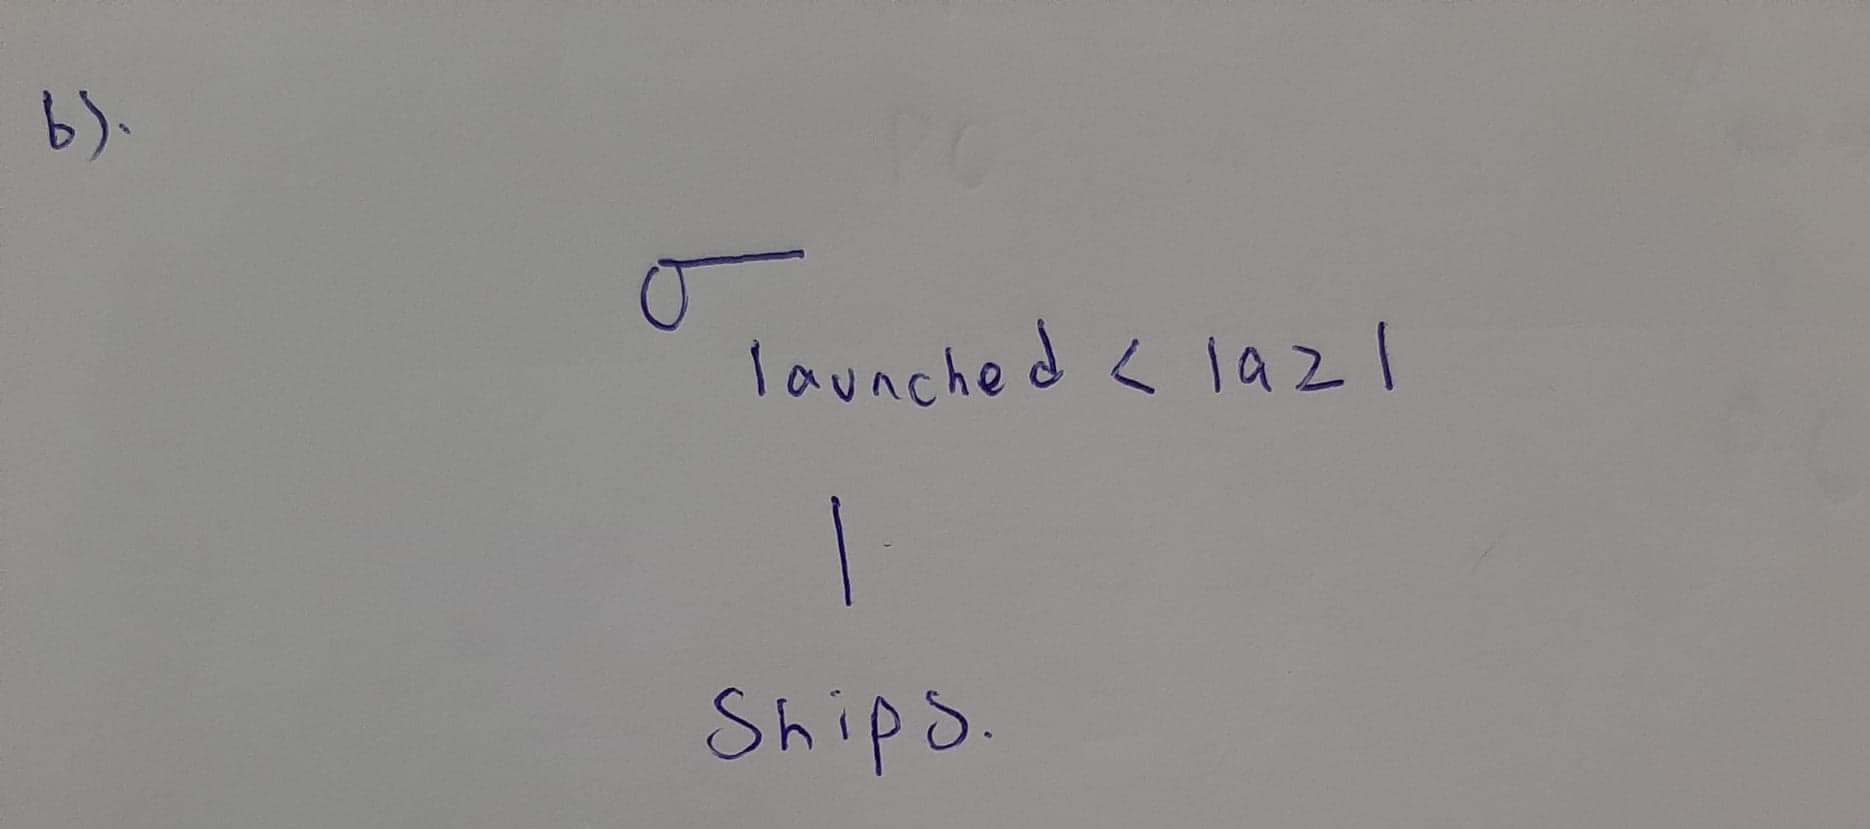
\includegraphics[width=0.7\linewidth]{images/worksheet_2_solution_18.jpg}
        \end{center}

        \item

        \textbf{Answer:}

        \bigskip

        \begin{center}
        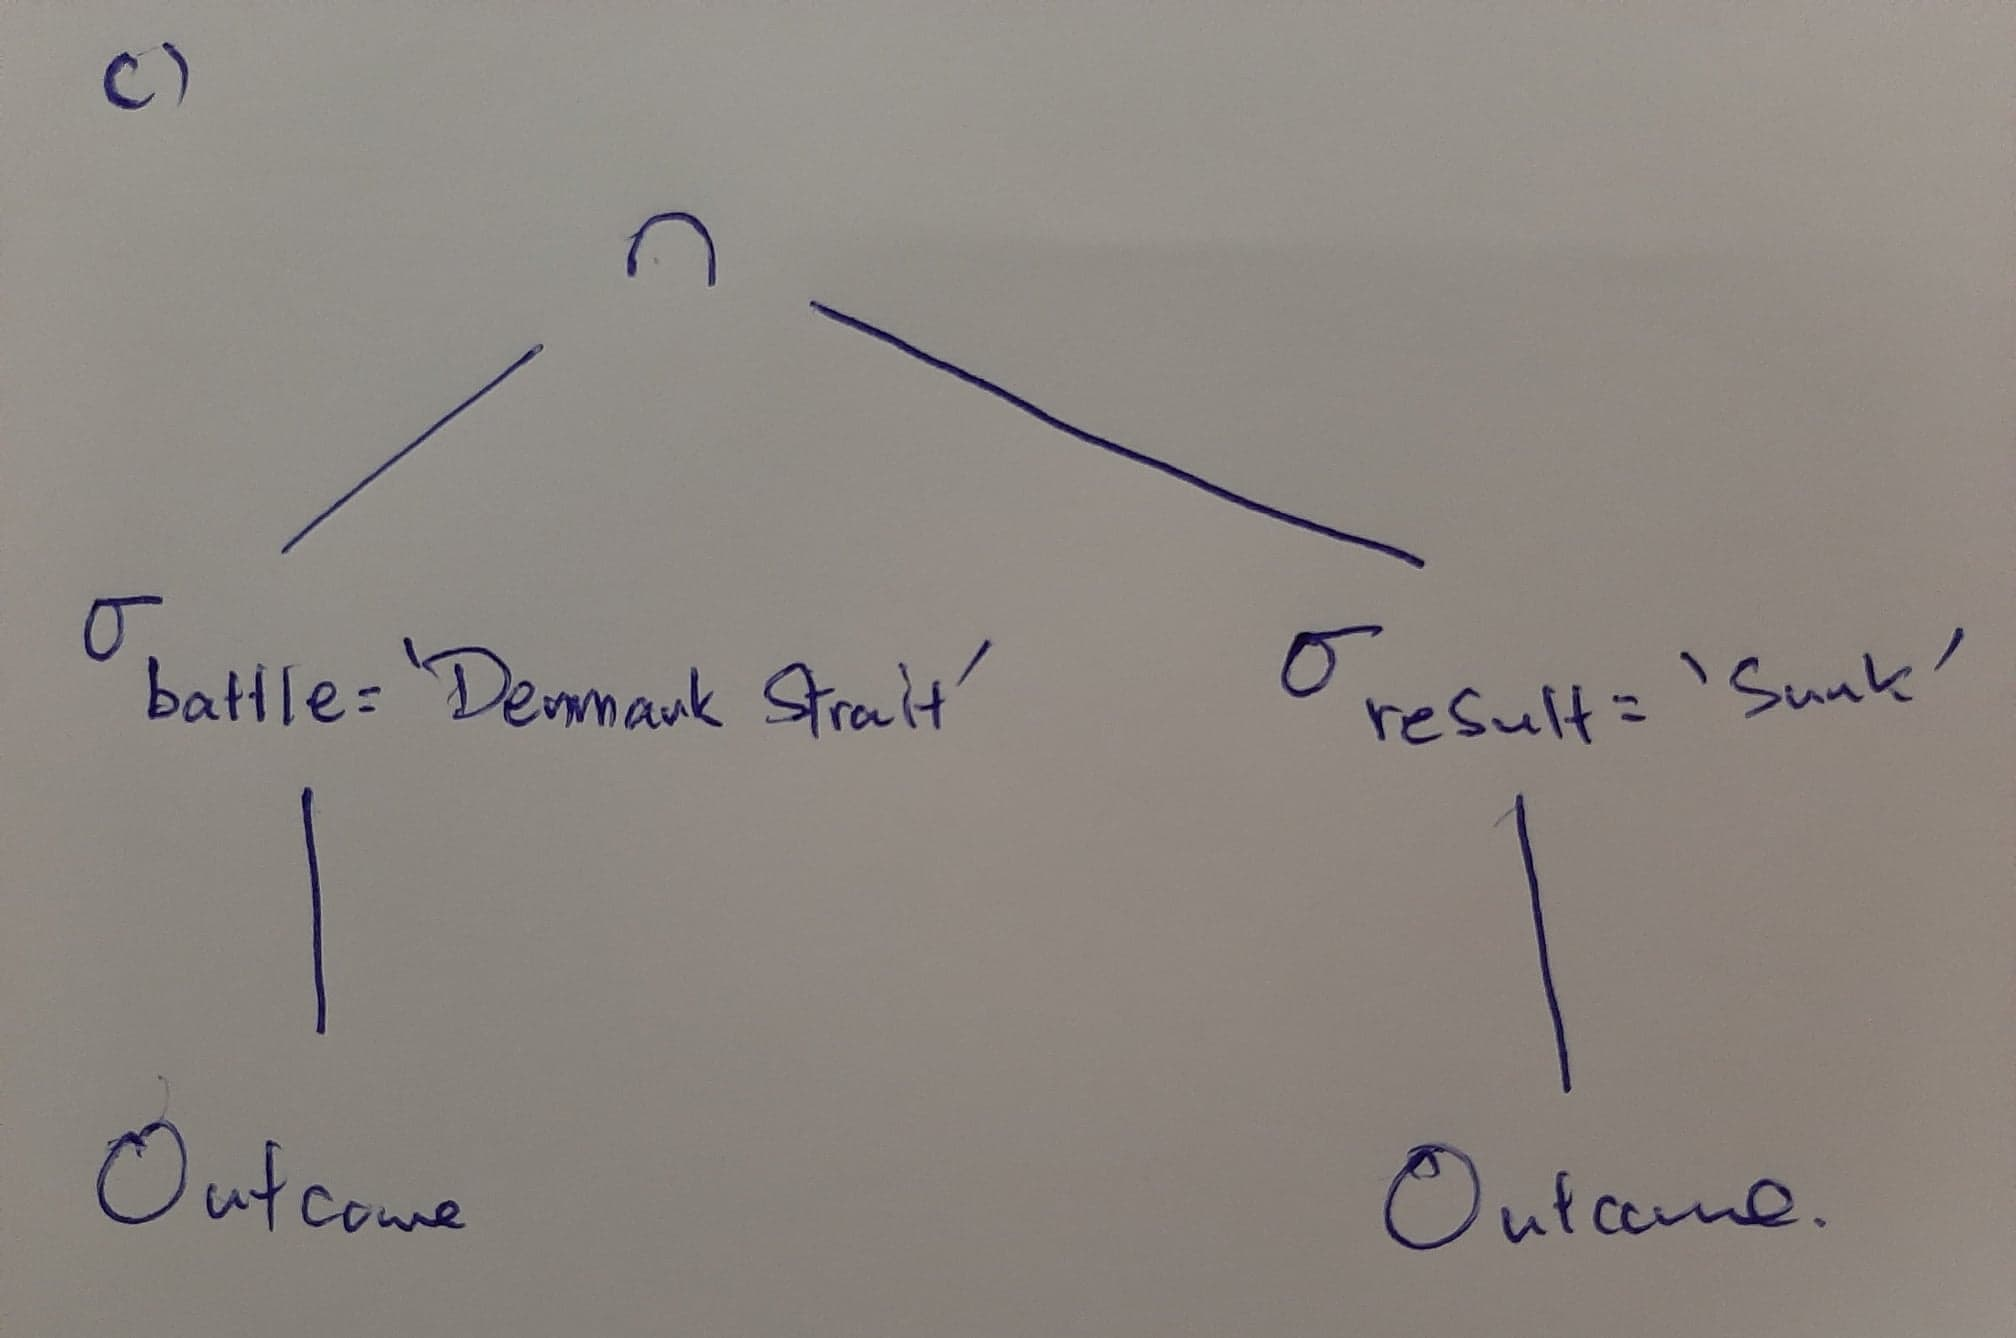
\includegraphics[width=0.7\linewidth]{images/worksheet_2_solution_19.jpg}
        \end{center}

        \item

        \textbf{Answer:}

        \bigskip

        \begin{center}
        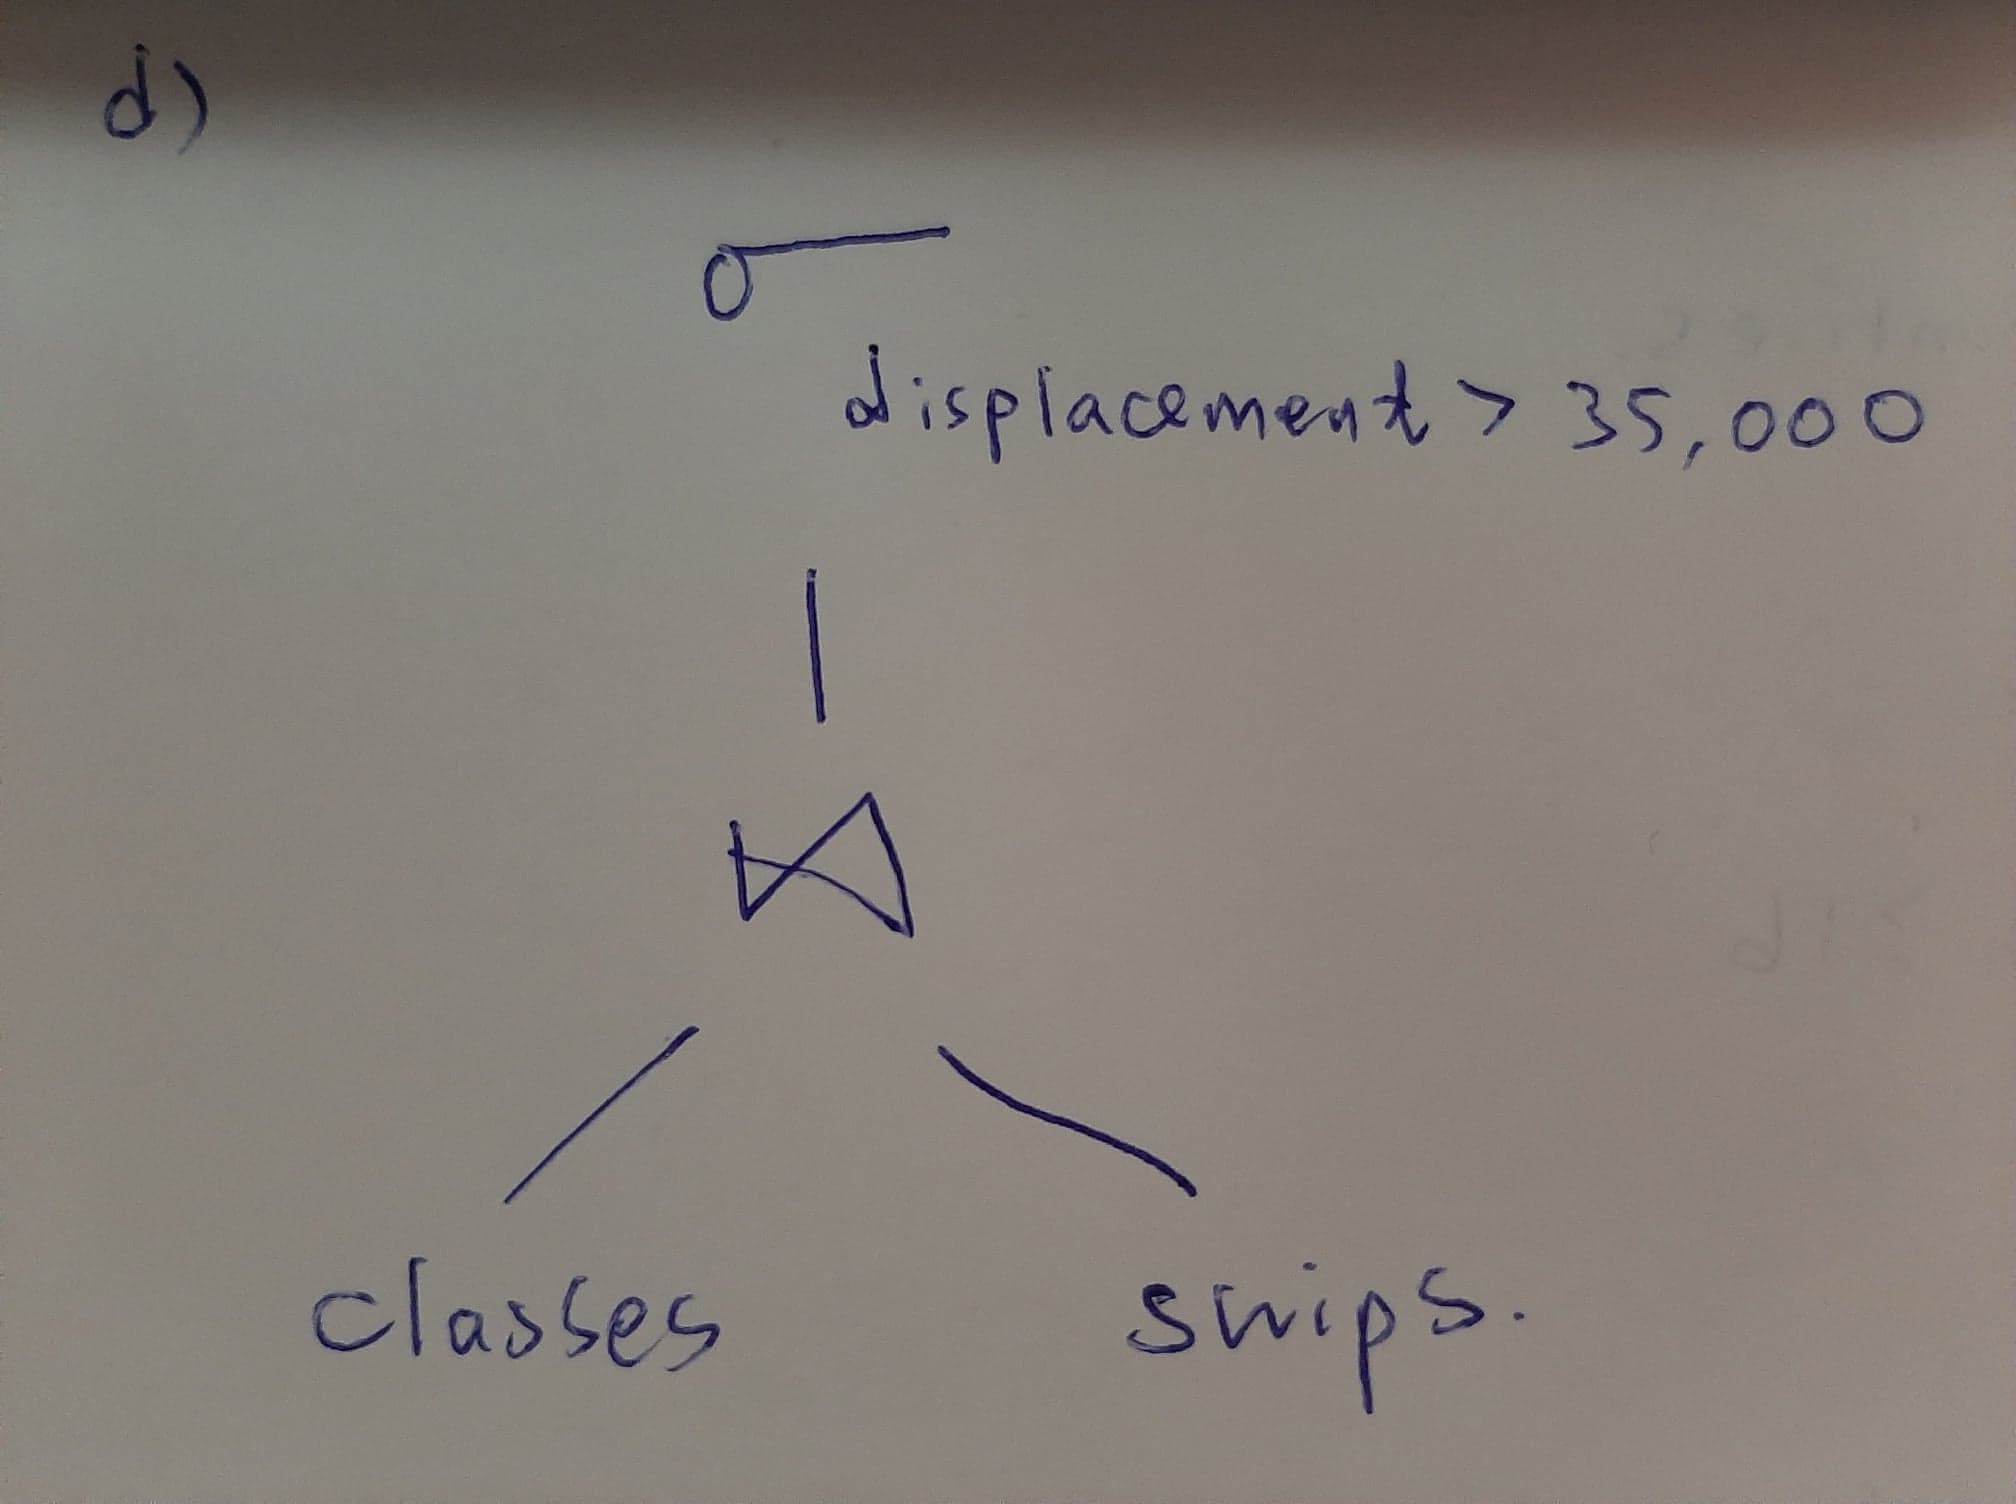
\includegraphics[width=0.7\linewidth]{images/worksheet_2_solution_20.jpg}
        \end{center}

        \item

        \textbf{Answer:}

        \bigskip

        \begin{center}
        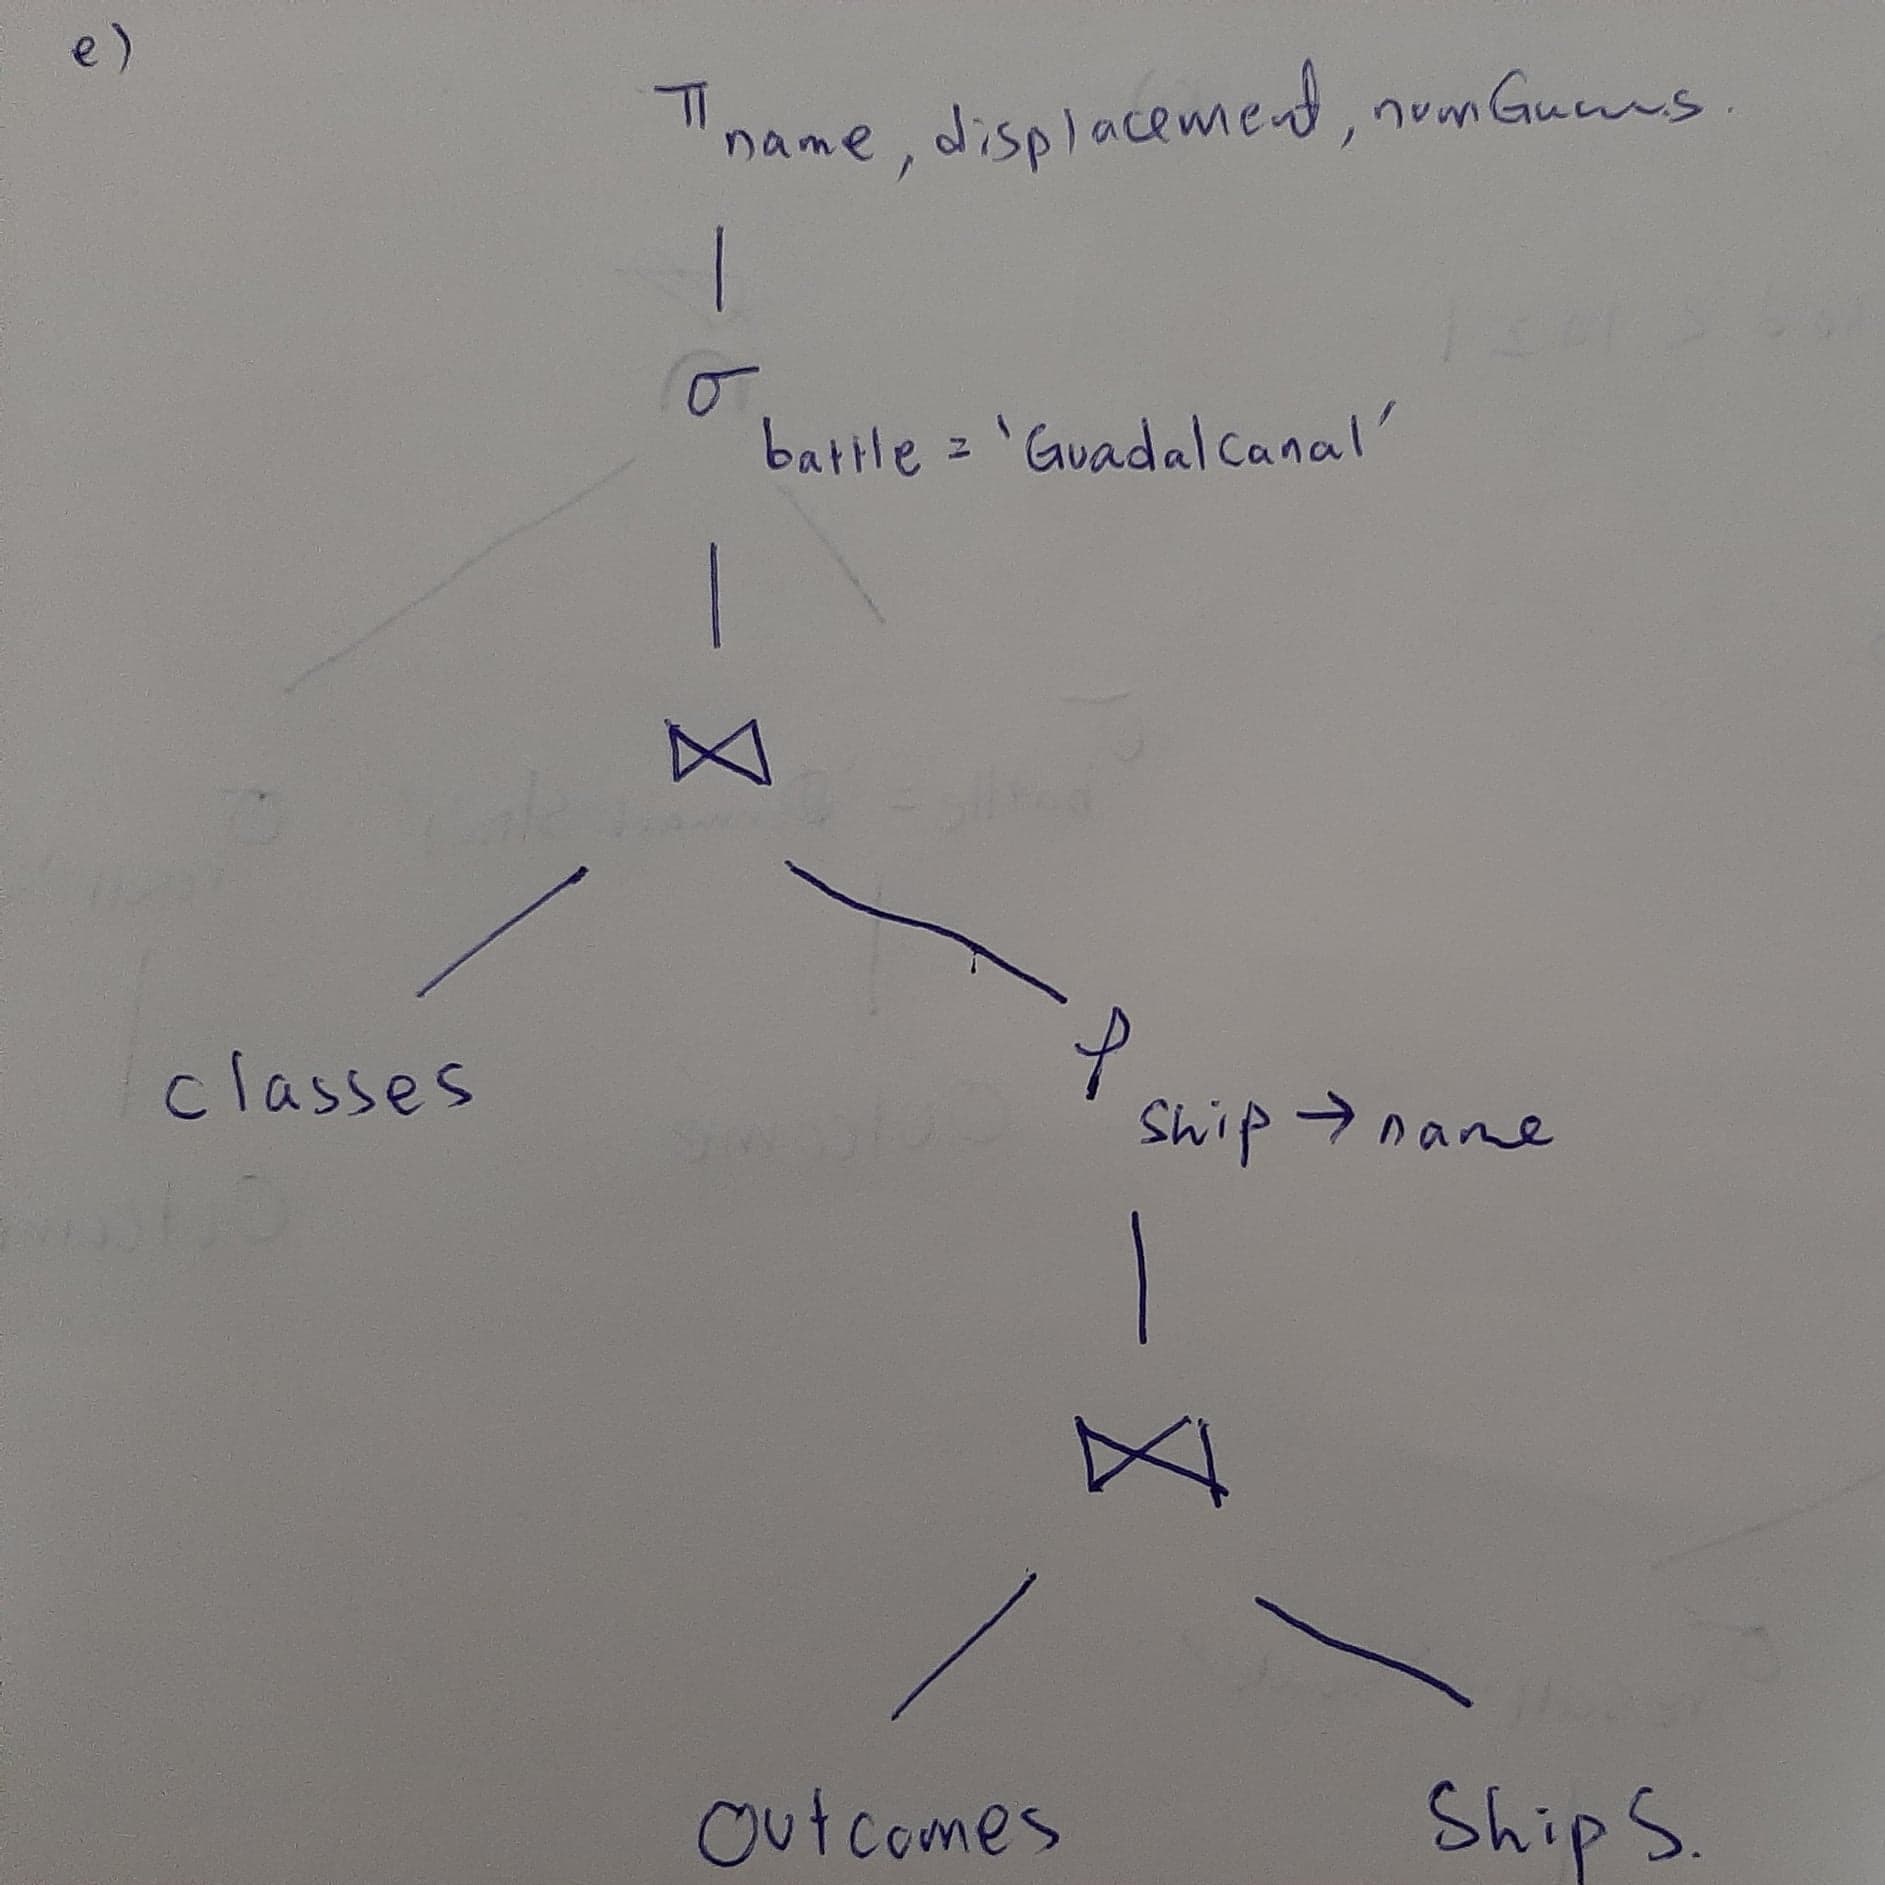
\includegraphics[width=0.7\linewidth]{images/worksheet_2_solution_21.jpg}
        \end{center}

        \item

        \textbf{Answer:}

        \bigskip

        \begin{center}
        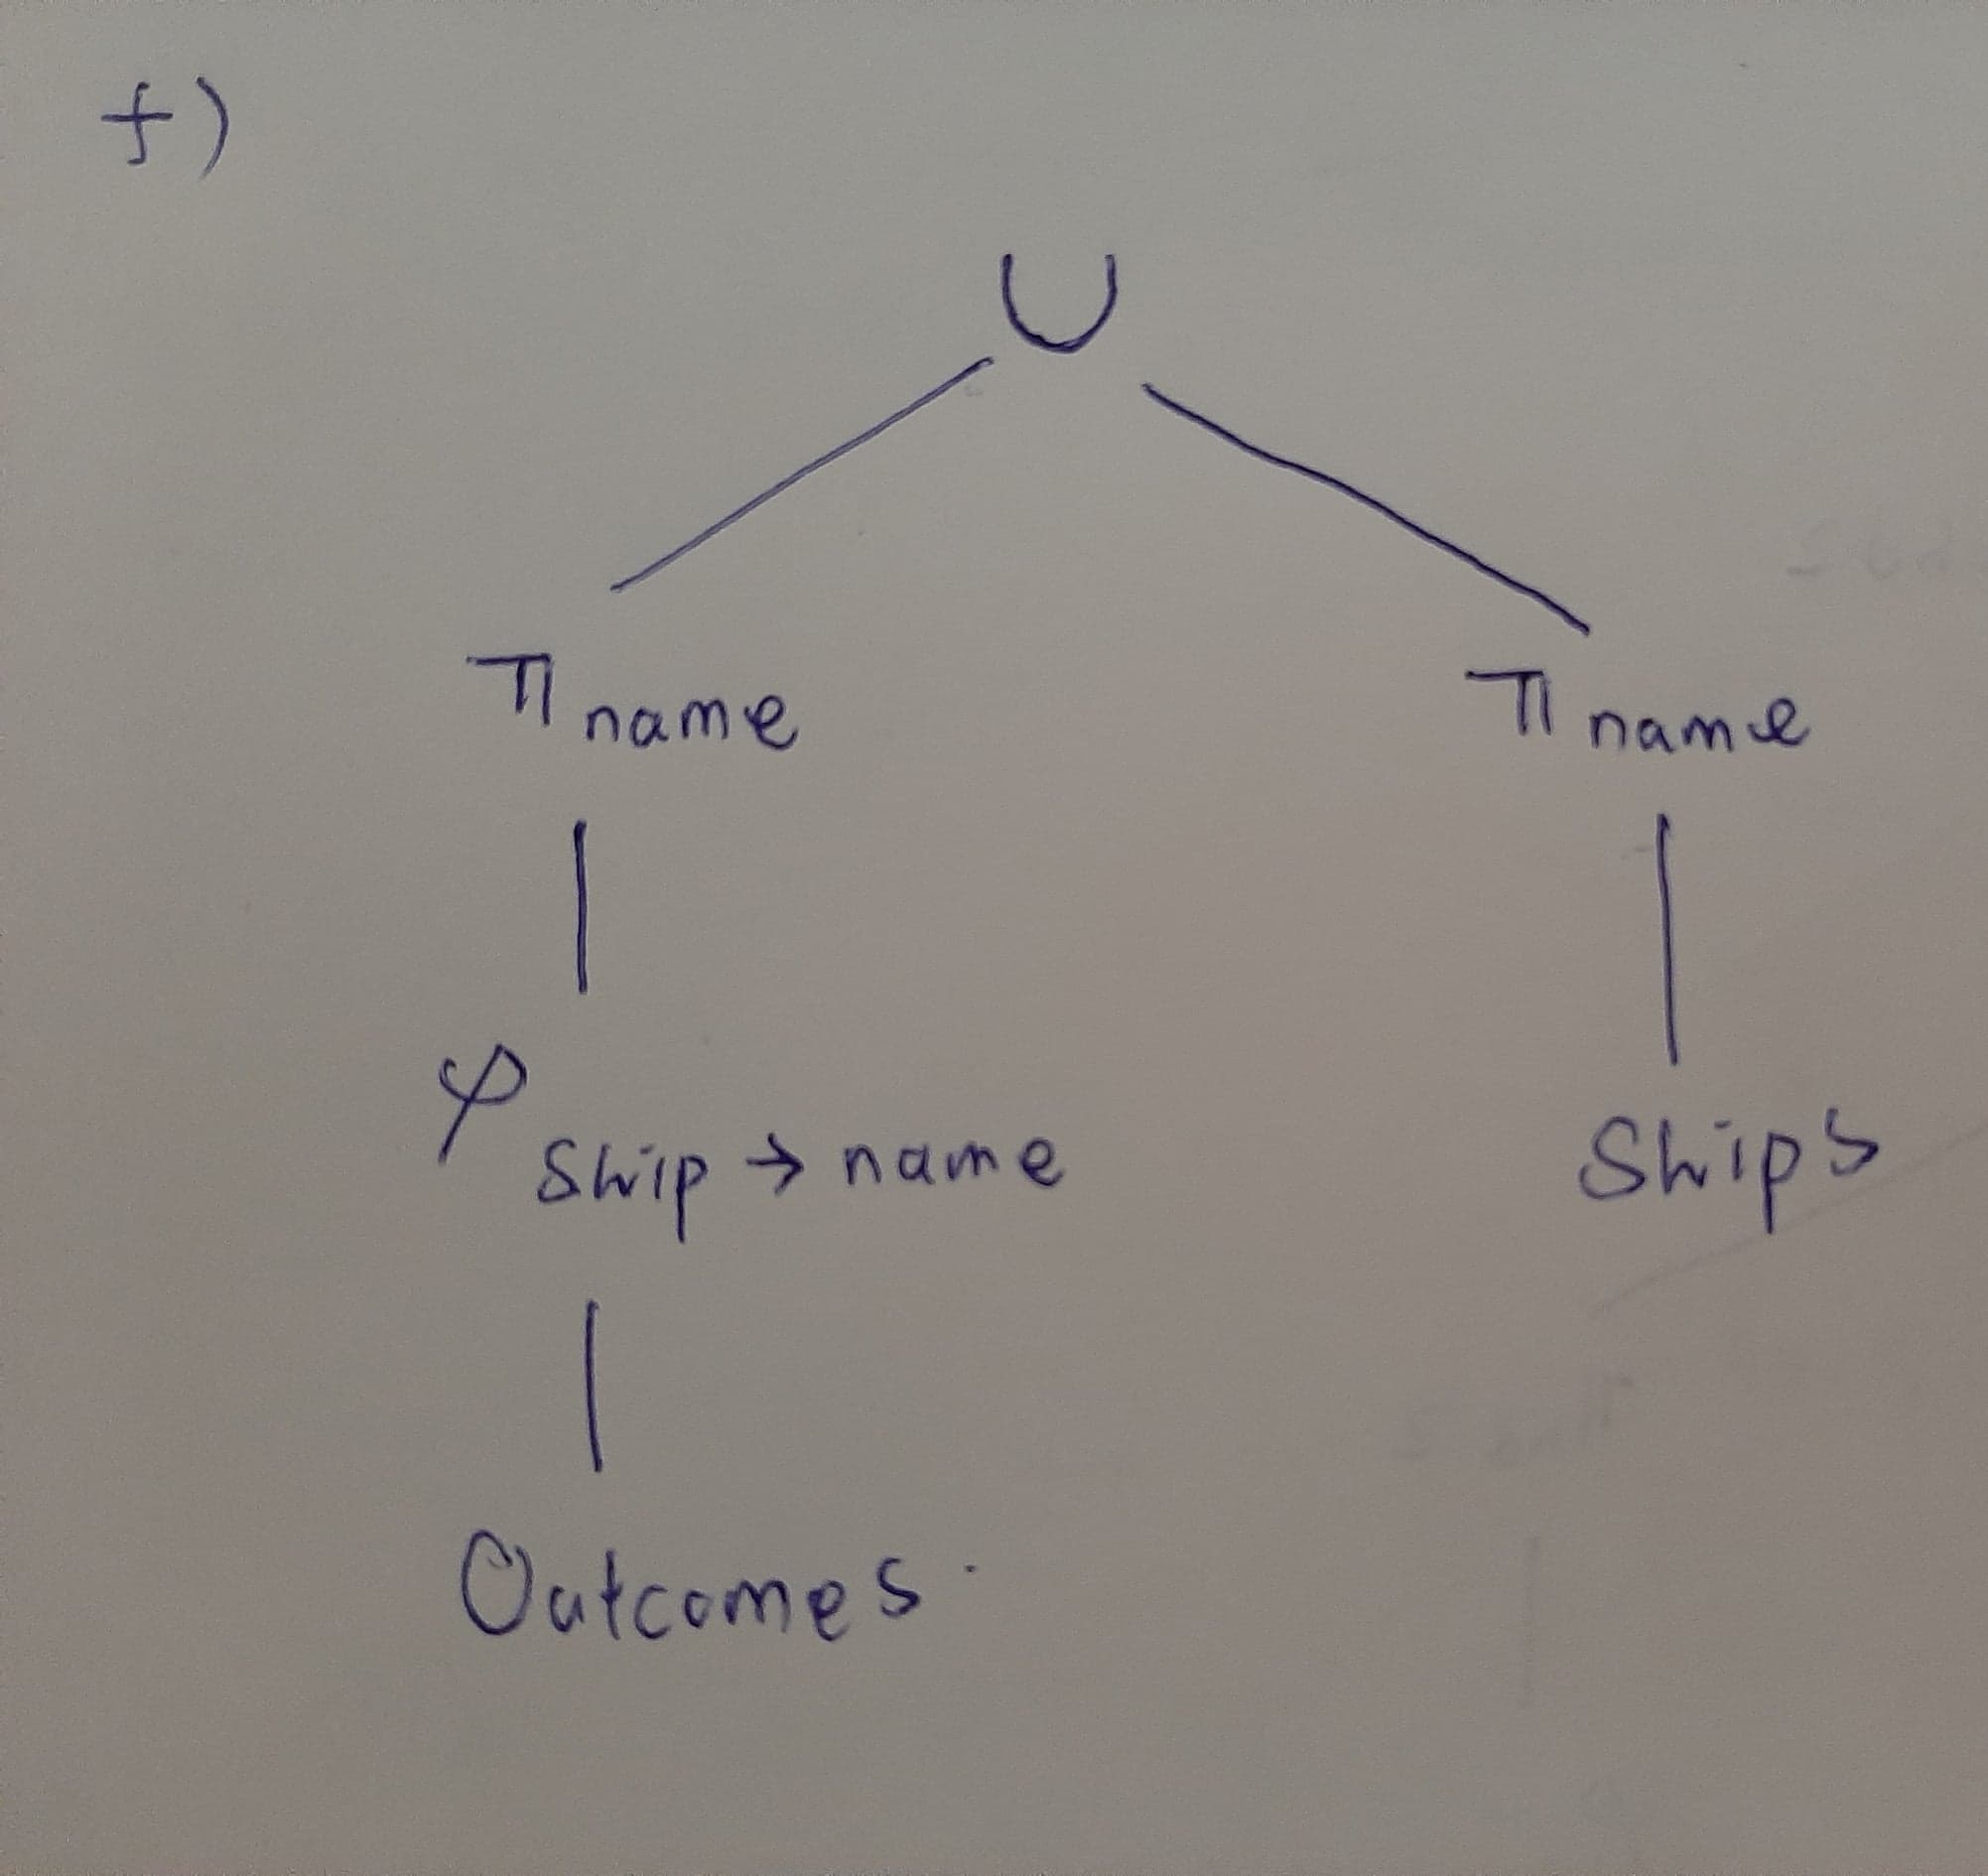
\includegraphics[width=0.7\linewidth]{images/worksheet_2_solution_22.jpg}
        \end{center}

        \item Omitted for now

        \item

        \textbf{Answer:}

        \bigskip

        \begin{center}
        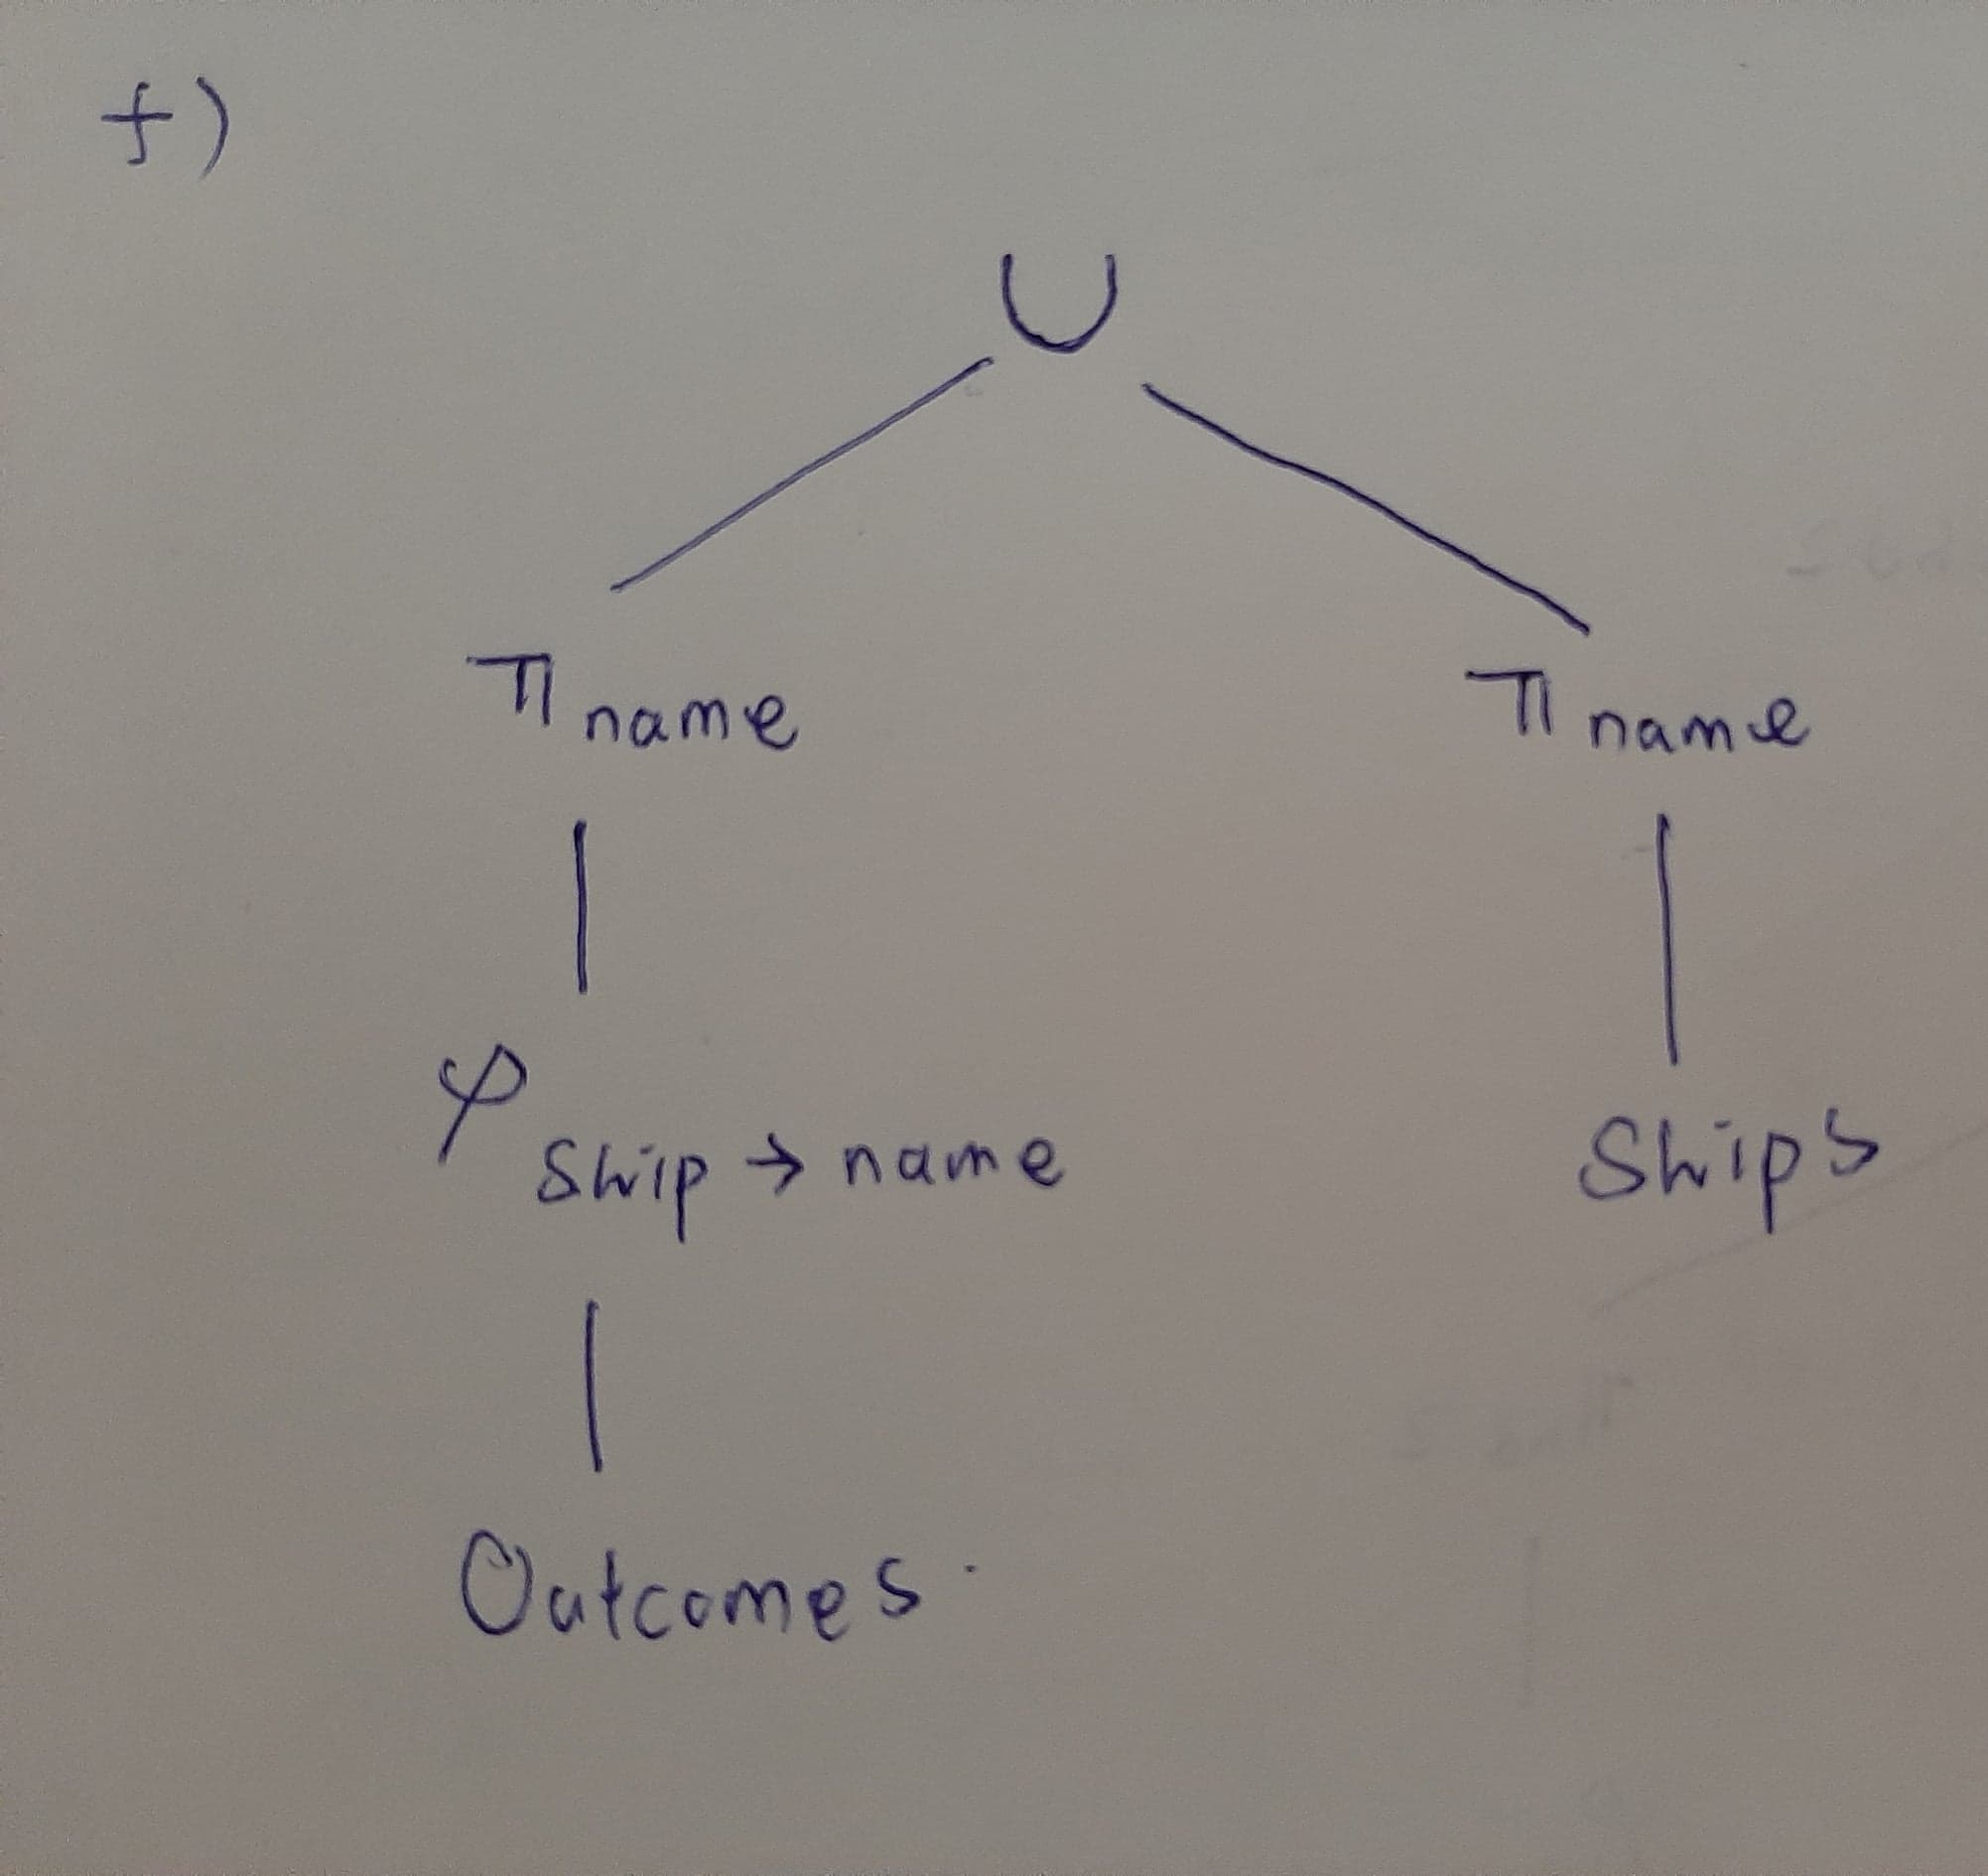
\includegraphics[width=0.7\linewidth]{images/worksheet_2_solution_22.jpg}
        \end{center}

        \item Omitted for now

    \end{enumerate}

    \item

    One difference exists in the number of attributes.

    \bigskip

    The definition of natural join (i.e. $\bowtie$) tells us a copy of duplicate attributes
    is eliminated.

    \bigskip

    Since $R$ and $S$ both have attribute $A$, the result $R \bowtie S$ would have one
    attribute of $A$.

    \bigskip

    On the other hand, the definition of theta join tells us $R \bowtie_C S$ is equivalent form
    of $\sigma_C(R \times S)$.

    \bigskip

    Since we know cross product doesn't eliminate duplicate attributes, the result
    $\sigma_{\text{R.A} = \text{S.A}}(R \times S)$ would have 2 attributes of $A$.

    \item


    \bigskip

    \underline{\textbf{Notes:}}

    \bigskip

    \begin{itemize}
        \item \textbf{Set:} is an unordered collection of elements without duplicates
        \item \textbf{Bags:} is unordered collection of elements with duplicates. A
        bag is also called \textbf{Multisets}
    \end{itemize}


\end{enumerate}

\end{document}